\documentclass[a4paper, 12pt]{scrreprt}
\usepackage[german]{babel}
\usepackage[german]{translator}
\usepackage[utf8]{inputenc}
\usepackage[T1]{fontenc}
\usepackage{ae}
\usepackage[bookmarks,bookmarksnumbered]{hyperref}
\usepackage{graphicx}
\usepackage{color}
\usepackage[dvipsnames]{xcolor}
\usepackage{booktabs}
%\usepackage{pdfpages}
%\usepackage[section]{placeins}

\newcommand{\col}[2]{\textcolor{#1}{#2}}

\begin{document}
	\thispagestyle{plain}

\begin{titlepage}
    \begin{center}
        
        \begin{figure}[ht]
        	\centering
        	
\includegraphics[width=0.66\textwidth, angle=0]{logo/name_blau_ofCourse.jpg}
        \end{figure}
        
    	\begin{title}
        	\title{\Huge{\textbf{Kurseinheiten-Manager \\ Entwurf\\}}}

		\end{title}
		\hspace{3cm}

        	Software Engineering Praktikum \\
        	Sommersemester 2015\\
        	Universität Passau\\


        	Betreuer: Andreas Stahlbauer \\
        	\hspace{1,5cm}\\
        	Version: 2.0 \\
        	\hspace{1,5cm}\\
        	Datum: 08.05.2015\\[50pt]
        	Team 3 \\
    
		    \ \\
        
        
        \begin{tabular}{ | l | l | l | l |}
            \hline
             \textbf{Matrikelnummer} & \textbf{Name} & \textbf{Phase} & \textbf{E-Mail}  \\ \hline
             63097 & Katharina Hölzl & Pflichtenheft & hoelzlka@fim.uni-passau.de \\ \hline
             64504 & Ricky Strohmeier& Entwurf & strohric@fim.uni-passau.de  \\ \hline
             64380 & Martin Bachhuber & Feinspezifikation  & bachhube@fim.uni-passau.de \\ \hline
             64080 & Tobias Fuchs & Implementierung  &  fuchstob@fim.uni-passau.de\\ \hline
             61085 & Sebastian Schwarz & Validierung & sebastian@nrschwarz.de \\ \hline  
             58379 & Patrick Cretu  &  Präsentation & cretu@fim.uni-passau.de \\ \hline
        \end{tabular}
        
        \ \\
        \ \\
        \hspace{3 cm}\\
        \textbf{Arbeitspakete Entwurf} \\
        \ \\
        
        \begin{tabular}{ | l | l |}
        	\hline
        	\textbf{Autor} & \textbf{Verantwortungsbereich} \\ \hline
        	Katharina Hölzl & Facelets  \\ \hline
        	Ricky Strohmeier& Facelets  \\ \hline
        	Martin Bachhuber & Einleitung, Systemarchitektur, Sequenzdiagramm  \\ \hline
        	Tobias Fuchs & Klassenbeschreibung, Klassendiagramm \\ \hline
        	Sebastian Schwarz & Klassenbeschreibung, Klassendiagramm, Systemfunktionen \\ \hline  
        	Patrick Cretu  &  ER-Modell, Sequenzdiagramm  \\ \hline
        \end{tabular}
        
    \end{center}
\end{titlepage}

% Platzierung des Änderungsdokumentes
\chapter*{Änderungsübersicht}
Änderungen gegenüber dem Pflichtenheft:
\begin{itemize}
	\item Ein registrierter Benutzer/Kursleiter kann sich selbst deaktivieren. Im System wird er dadurch auf inaktiv gesetzt. Eine endgültige Löschung aus dem System kann nur der Administrator vornehmen.
	\item Ein Kursleiter kann für einen Kurs mehrere regelmäßige Kurseinheiten auf einmal anlegen.
	\item Ein Kursleiter kann die regelmäßigen Kurseinheiten eines Kurses auf einmal bearbeiten.
\end{itemize} 

% Platzierung des Inhaltsverzeichnisses
\tableofcontents

\chapter{Einleitung}
\begin{tiny}
MB \\
\end{tiny}
In diesem Dokument wird der grundlegende Entwurf der Webanwendung \glqq ofCourse\grqq{} dargestellt. Diese Webapplikation soll es Betreibern verschiedensten Fachbereichen erleichtern ihre Veranstaltungen zu organisieren, sowie zu planen. Des Weiteren können sich Nutzer von \glqq ofCourse\grqq{} über jene Veranstaltungen bzw. Kurse leicht informieren und anmelden. Im Laufe dieses Dokuments wird auf die Architektur des Systems, die verwendeten Design Patterns und die Fehlerbehandlungen eingegangen. Im Klassendiagramm werden die einzelnen Klassen des Systems, sowie die Pakete präsentiert. Eine genauere Erklärung der View wird im Kapitel der Facelets und deren jeweiligen Elemente diskutiert. In den Systemfunktionen werden grundlegende Aktionen, wie Email-Versand erläutert, sowie der Umgang mit Fehlern. Zum besseren Verständnis des Datenfluss wird jeweils ein Sequenzdiagramm bezüglich einer typischen Aktion in der Applikation veranschaulicht. 
Am Ende dieser Entwurfsbeschreibung wird das verwendete Datenbankschema mithilfe eines ER-Modells graphisch dargestellt.

\chapter{Systemarchitektur}
\begin{tiny}
MB
\end{tiny}
\section{Schichtenarchitektur}
	Um die Systemarchitektur von \glqq ofCourse\grqq{} besser zu veranschaulichen soll folgende Schichtenarchitektur dienen. Diese baut auf das Prinzip des Entwurfsmusters \glqq Model 2\grqq{} auf. \\ \\
    %Bild der Schichtenarchitektur
    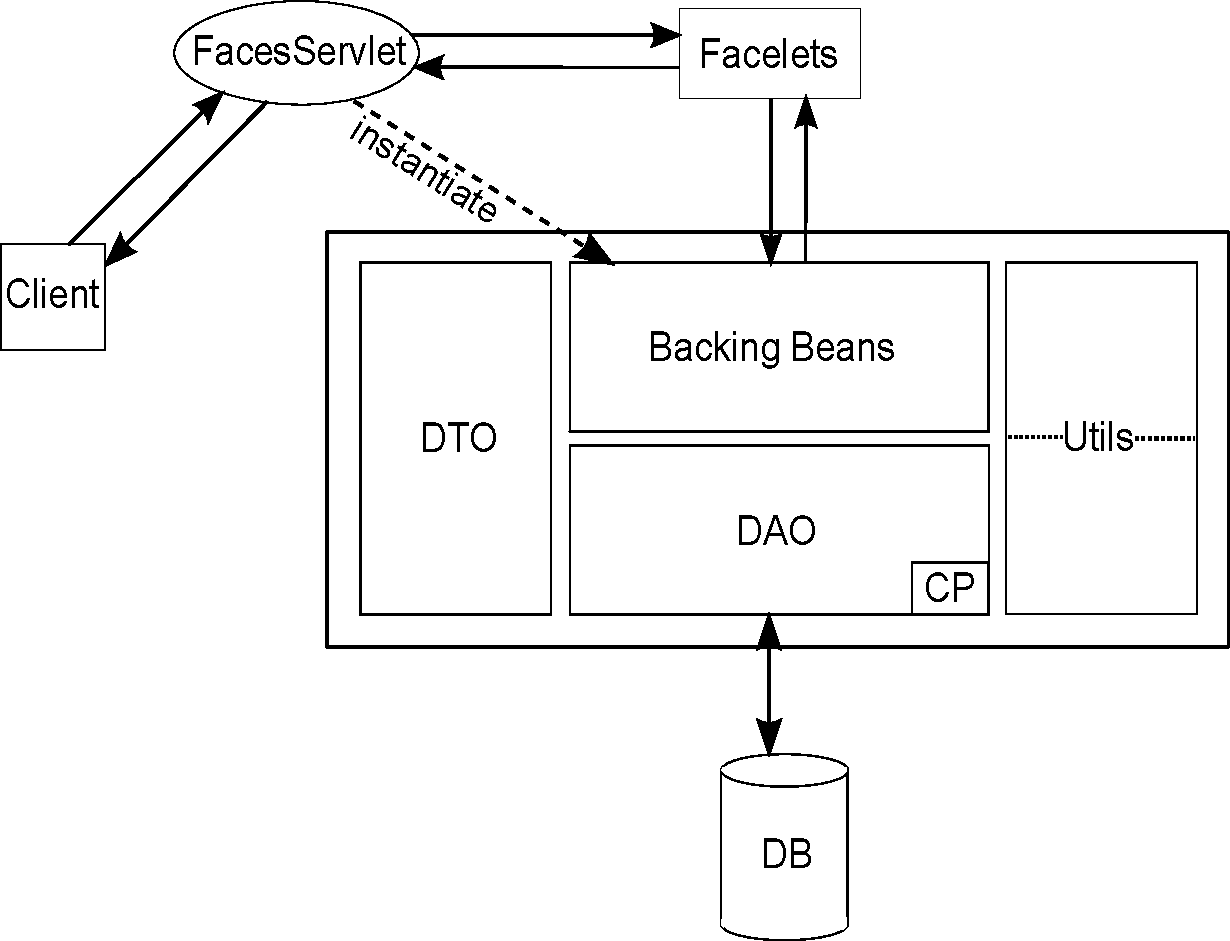
\includegraphics[scale=0.50]{Grafiken/Schichtenarchitektur.pdf}
	\subsection{Faces-Servlet}
	    Das Faces-Servlet fungiert im System als Controller, der eine HTTP-Request abfängt, diese bearbeitet, sowie weiterleitet. Das Faces-Servlet muss in jeder JSF-Applikation vorhanden sein und wird dementsprechend in der Webkonfigurationsdatei \textit{web.xml} definiert bzw. konfiguriert. 
    \subsection{Facelets}
    	Die View wird durch Facelets repräsentiert. Sie stellen die Inhalte dar, der vom Controller übergeben wird. Des Weiteren werden in der View die Benutzerinteraktionen entgegengenommen. Genauer auf Facelets wird unter Kapitel 4 Facelets eingegangen.
   	\subsection{Model}
   	Das Model kann in vier Bereiche unterteilt werden. Zunächst gäbe es die \glqq Upper Layer\grqq{}, welche die Backing Beans beinhalten, die \glqq Lower Layer\grqq{} mit den Data Access Objects (DAOs) und dem Connection Pool (CP), des Weiteren gäbe es noch die Data Transfer Objects (DTOs) und die Utils. 
   		\subsubsection{Upper Layer}
   		Die \glqq Upper Layer\grqq{} besteht aus den Backing Beans. In Diesen ist zum Einen die Geschäftslogik enthalten, zum Anderen werden dort die überlieferten Benutzereingaben der Facelets übergeben, weiterverarbeitet und gespeichert. Die Backing Beans werden in der zentralen JSF-Konfigurationsdatei \textit{faces-config.xml} verwaltet.
    	\subsubsection{Lower Layer}
    	In der \glqq Lower Layer\grqq{} befinden sich die Data Access Objects und der Connection Pool. Mithilfe der im CP lagernden Datenbankverbindungen greifen die DAOs auf die darunterliegende Database (DB) zu.
    	\subsubsection{DTO}
    	Die Data Transfer Objects dienen als Schnittstelle zwischen den Backing Beans und den zugehörigen DAOs. Sie bündeln logisch zusammenhängende Daten in einem Objekt, um zeitintensive Fernzugriffe durch einen zu ersetzen.
    	\subsubsection{Utils}
    	Utils fungieren als Hilfs- und Verwalterklasse. Die Utils werden auch wiederum unterteilt, die man entweder den Backing Beans oder den DAOs zuordnen kann. 
    \subsection{Database}
    Für die persistente Speicherung von Daten ist die Database (DB) zuständig. Dort werden Daten wie z.B. \textit{BenutzerID, Benutzername, Kurseinheit, Kurslehrer} etc. gespeichert. Zugriff auf die DB haben nur die DAOs. 

\section{Package-Diagramm}
 Um einen kleinen Überblick der verwendeten Packages im System zu bekommen, soll die folgende Figur dazu Abhilfe schaffen. \\ \\
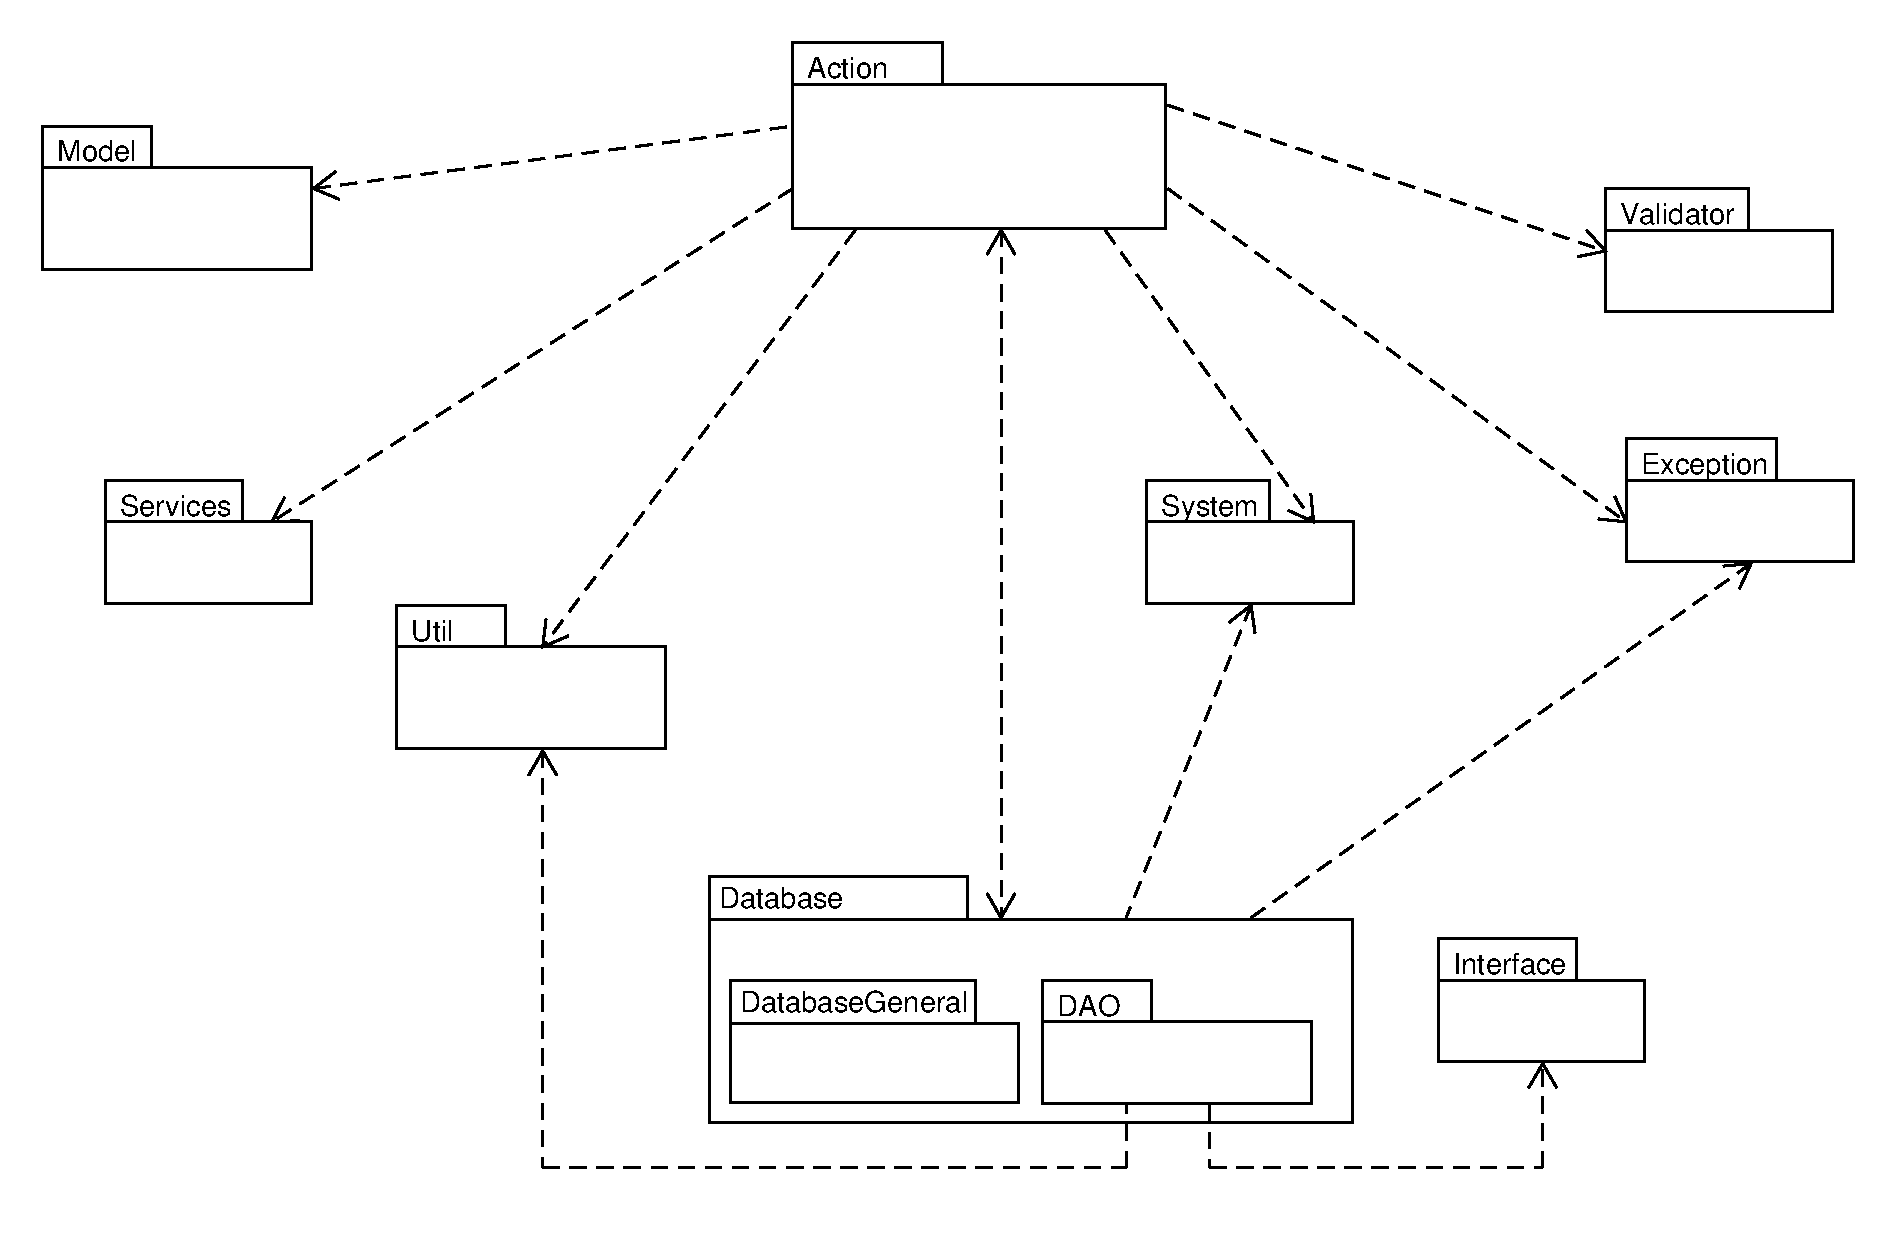
\includegraphics[scale=0.45]{Grafiken/PackageDiagramm.pdf}      
    
\section{Design Patterns}
Damit keine wiederkehrenden Entwurfsprobleme bei der Softwareentwicklung auftreten, werden bewährte Lösungsansätze, die sogenannten \glqq Design Patterns\grqq{}, benutzt. Sie dienen dazu den Entwurf möglichst flexibel, erweiterbar und auch einfach zu gestalten. Aufgrund dessen werden im Nachfolgendem die für das System eingesetzten \textit{Design Patterns} beschrieben:
	\begin{itemize}
%		\item \textbf{Model 2:} Bei dem Architekturmuster \textit{Model 2} wird die View (Facelets) von der Geschäftslogik (Backing Beans) bei einer Java-Webapplikation getrennt. Der Ablauf sieht im Groben so aus, dass ein HTTP-Request eines Clients an den Controller (Faces-Servlet) weitergeleitet wird. Darauffolgend \glqq steuert\grqq{} der Controller alle notwendigen Schritte zur Beschaffung des Inhalts für die Darstellung. Der Controller legt den Inhalt in einer Backing Beans ab und entscheidet, welcher View der Inhalt übergeben wird. Die View wiederum stellt den Inhalt dar, der vom Controller weitergereicht wurde.
		\item \textbf{Data Transfer Object:} Das DTO fasst mehrere Daten in einem Objekt zusammen, damit sie in einem Aufruf übergeben werden. Somit können Datensätze durch die Schichten transportiert werden.
		\item \textbf{Dependency Injection:} Dependency Injection ist ein JSF Standard, um Backing Beans zu verwalten. Hierbei werden die benötigten Objekte an einem zentralen Ort hinterlegt, was auch die Flexibilität erhöht.  
		\item \textbf{Creational Pattern:} Die Creational Patterns sind eine Teilmenge der Design Patterns und dienen als Entwurfsmuster für die Erzeugung von Objekten. Man kann diese in folgende Pattern unterscheiden.
			\begin{itemize}
				\item \textbf{Factory Pattern:} Bei diesem Pattern werden mehrere ähnliche Objekte durch Aufruf einer Methode anstatt durch direkten Aufruf eines Konstruktors erzeugt.
				\item \textbf{Object Pooling:} Beim Object Pooling werden ressourcenintensive Objekte (hier Datenbankverbindungen) in einem Pool (Connection Pool) bereitgehalten, um sie bei Bedarf erneut nutzen zu können, was sich wiederum positiv auf die Ausführungszeit auswirkt.
				\item \textbf{Singleton:} Es soll sichergestellt werden, dass von einem Objekt jeweils nur eine Instanz existiert. Diese sind darüber hinaus global verfügbar.  
			\end{itemize}
	\end{itemize}
\section{Einsatz externer Libraries}
Es werden im System auf bereits vorhandenen Libraries zurückgegriffen.
	\begin{itemize}
		\item \textbf{PostgreSQL JDBC 9.4-1201:} Der PostgreSQL JDBC-Treiber wird für die Kommunikation mit der Datenbank verwendet.
		\item \textbf{JSF 2.2:} Für die Implementierung von JSF wird das Framework Mojarra 2.2.10 benutzt.
		\item \textbf{JavaMail API 1.5.2:} Library für das Versenden von Emails.
		\item \textbf{Bootstrap 3.3.0:} Bootstrap dient als Grundlage für das Design der Facelets.
		\item \textbf{Tomcat 8.0.21:} Webcontainer, um die in Java geschriebenen Webapplikationen auszuführen.
		\item \textbf{Log4J:} Library für das Loggen von Meldungen.
	\end{itemize}
\section{Fehlerbehandlung}
	\subsection{Nicht-Autorisierter Zugriff}
	Sofern der User eine Aktion ausführen will, aber nicht die entsprechenden Rechte dafür besitzt, wird eine Fehlermeldung ausgegeben. Beispielsweise will sich ein Gast bestimmte Details eines Kurs anzeigen lassen, was aber nur registrierten Usern vorbehalten ist. Dem Gast wird eine Fehlermeldung angezeigt und gegebenenfalls auf die Login Seite verwiesen. Zur Realisierung hierfür werden die Facelets von einem Phaselistener überprüft.
	\subsection{Fehlerhafte Benutzereingaben}
	Wenn ein Gast sich registrieren will, aber in den Formulardaten eine ungültige Eingabe tätigt, so soll der Gast nicht alles neu eingeben müssen, sondern nur die fehlerhaften Stellen. Der Fehler wird auf derselben Seite angezeigt, somit wird keine Fehler-Seite extra benötigt.
	\subsection{Exceptions}
	Sollten Fehler auftreten auf die der User keinen Einfluss hat, so wird der Nutzer auf eine Fehler-Seite geleitet. Auf dieser Seite befinden sich Informationen zu dem Fehler und es wird eine weitere Vorgehensweise zur Verfügung gestellt. Bestimmte Exceptions wie beispielsweise eine SQL-Exception, die in der DAO Schicht auftreten kann, werden gefangen und geworfen, indem globale Exception-Handler implementiert werden (Kapitel 3.8.6 InvalidDBTransferException). Bei kritischen Exceptions wird auch ein Logfile angefertigt, um im Nachhinein genau zu verfolgen können wo und wann der Fehler aufgetreten ist.
	\subsection{HTTP-Statuscodes}
	Für den User werden HTTP-Statuscodes generiert. Somit bleiben kryptische Fehlermeldungen dem User verborgen. Dieser Fehler kann bei Problemen seitens des Webservers auftreten. Dem User werden die Fehler auf einer neuen Seite angezeigt: \\ \\
	\begin{tabular}{|l|l|}
		\hline
		Status Code & Beschreibung \\
		\hline
		403 & Zugriff nicht autorisiert \\
		404 & Datei/Ressource nicht vorhanden \\
		408 & Server-Timeout \\
		500 & Interner Server Fehler \\
		503 & Server nicht erreichbar \\
		\hline
 	\end{tabular}		     


\chapter{Klassenbeschreibung und Klassendiagramm}
	\newcommand{\class}[1]{\paragraph{Klasse #1:}\ \\ }
	\newcommand{\interface}[1]{\paragraph{Interface #1:}\ \\ }
	\newcommand{\method}[1]{\textcolor{blue}{#1}}
	\newcommand{\kursiv}[1]{{\it #1}}
	\newcommand{\override}{{\it @Override}\ \\}
	
	Dieses Kapitel dient der Aufführung der Klassenbeschreibung und der Darstellung des UML - Klassendiagramms der Anwendung \textbf{ofCourse}.
	Um eine bessere Übersicht und Strukturierung zu erhalten, wird das ganze Projekt in Packages aufgeteilt.\\
	Die Packagestruktur ist wie folgt aufgebaut: de.ofCourse.PACKAGENAME.\\
	\ \\
	Eine detaillierte Beschreibung der Klassen ist in dem beigefügten Dokument \kursiv{Klassenbeschreibung ofCourse} zu finden.\\
	\ \\
	Die verwendeten Synchronizations, Injections und Scopes werden im Folgenden kurz zusammenfassend
	beschrieben.\\
	\begin{itemize}
		\item \textbf{Synchronizations}\\
		Die Anwendung \textbf{ofCourse} kommt, mit einer einzigen Ausnahme ohne den Modifier \kursiv{synchronized} aus. Diese Ausnahme stellt die Klasse \kursiv{DatabaseConnectionManager} mit ihren Methoden \kursiv{getConnection()}  und \kursiv{releaseConnection()} dar.
		\item \textbf{Injections}\\
		Alle Klassen des Package \kursiv{action}, außer die Klasse \kursiv{SessionUserBean} und die Klasse
		\kursiv{MailBean}  enthalten ein \kursiv{private SessionUserBean sessionUser} Attribut, welches mit \kursiv{@ManagedProperty("\#sessionUser")} gekennzeichnet
		ist. Somit wird in diese Klassen die \kursiv{SessionUserBean} Klasse
		über Injection eingebunden.
		In der Klasse \kursiv{ContactUsersBean} wird zusätzlich zu der oben genannten Injection noch die Klasse \kursiv{MailBean}
		eingebunden.
		\item \textbf{Scopes} \\
		Alle Klassen des Package \kursiv{action} haben Scopes. Zusätzlich hat auch noch die Klasse \kursiv{LaunchSystem} aus dem Package \kursiv{system} einen Scope. Sie ist neben der Klasse \kursiv{MailBean} die einzige Klasse, welche mit \kursiv{@ApplicationScoped} annotiert ist.\\ Die Klasse \kursiv{SessionUserBean}, welche die Informationen der Session des Users speichert, ist systemweit die einzige Klasse, welche die Annotation \kursiv{@SessionScoped}  besitzt.\\ Alle Klassen, die die Funktionalität von Pagination implementieren, besitzen die Annotation \kursiv{@ViewScoped}.\\ Die restlichen Klassen, die einen Scope besitzen, sind alle mit \kursiv{@RequestScoped} annotiert.
	\end{itemize}
	
	
	\section{Klassendiagramm}
	\begin{tiny}
		Diagramm: SeSc und TF\\
	\end{tiny}\\
	Aus Gründen der Übersichtlichkeit im gesamten Klassendiagramm und da das Interface \kursiv{Transaction} und die damit verbundene Vergabe von Verbindungen zur Datenbank für unser System spezifisch ist, wird dieses exemplarisch in einem separaten Beispielfall in einem Klassendiagramm \ref{fig:Teildiagramm} dargestellt.
	\begin{figure}[h]
	\centering
	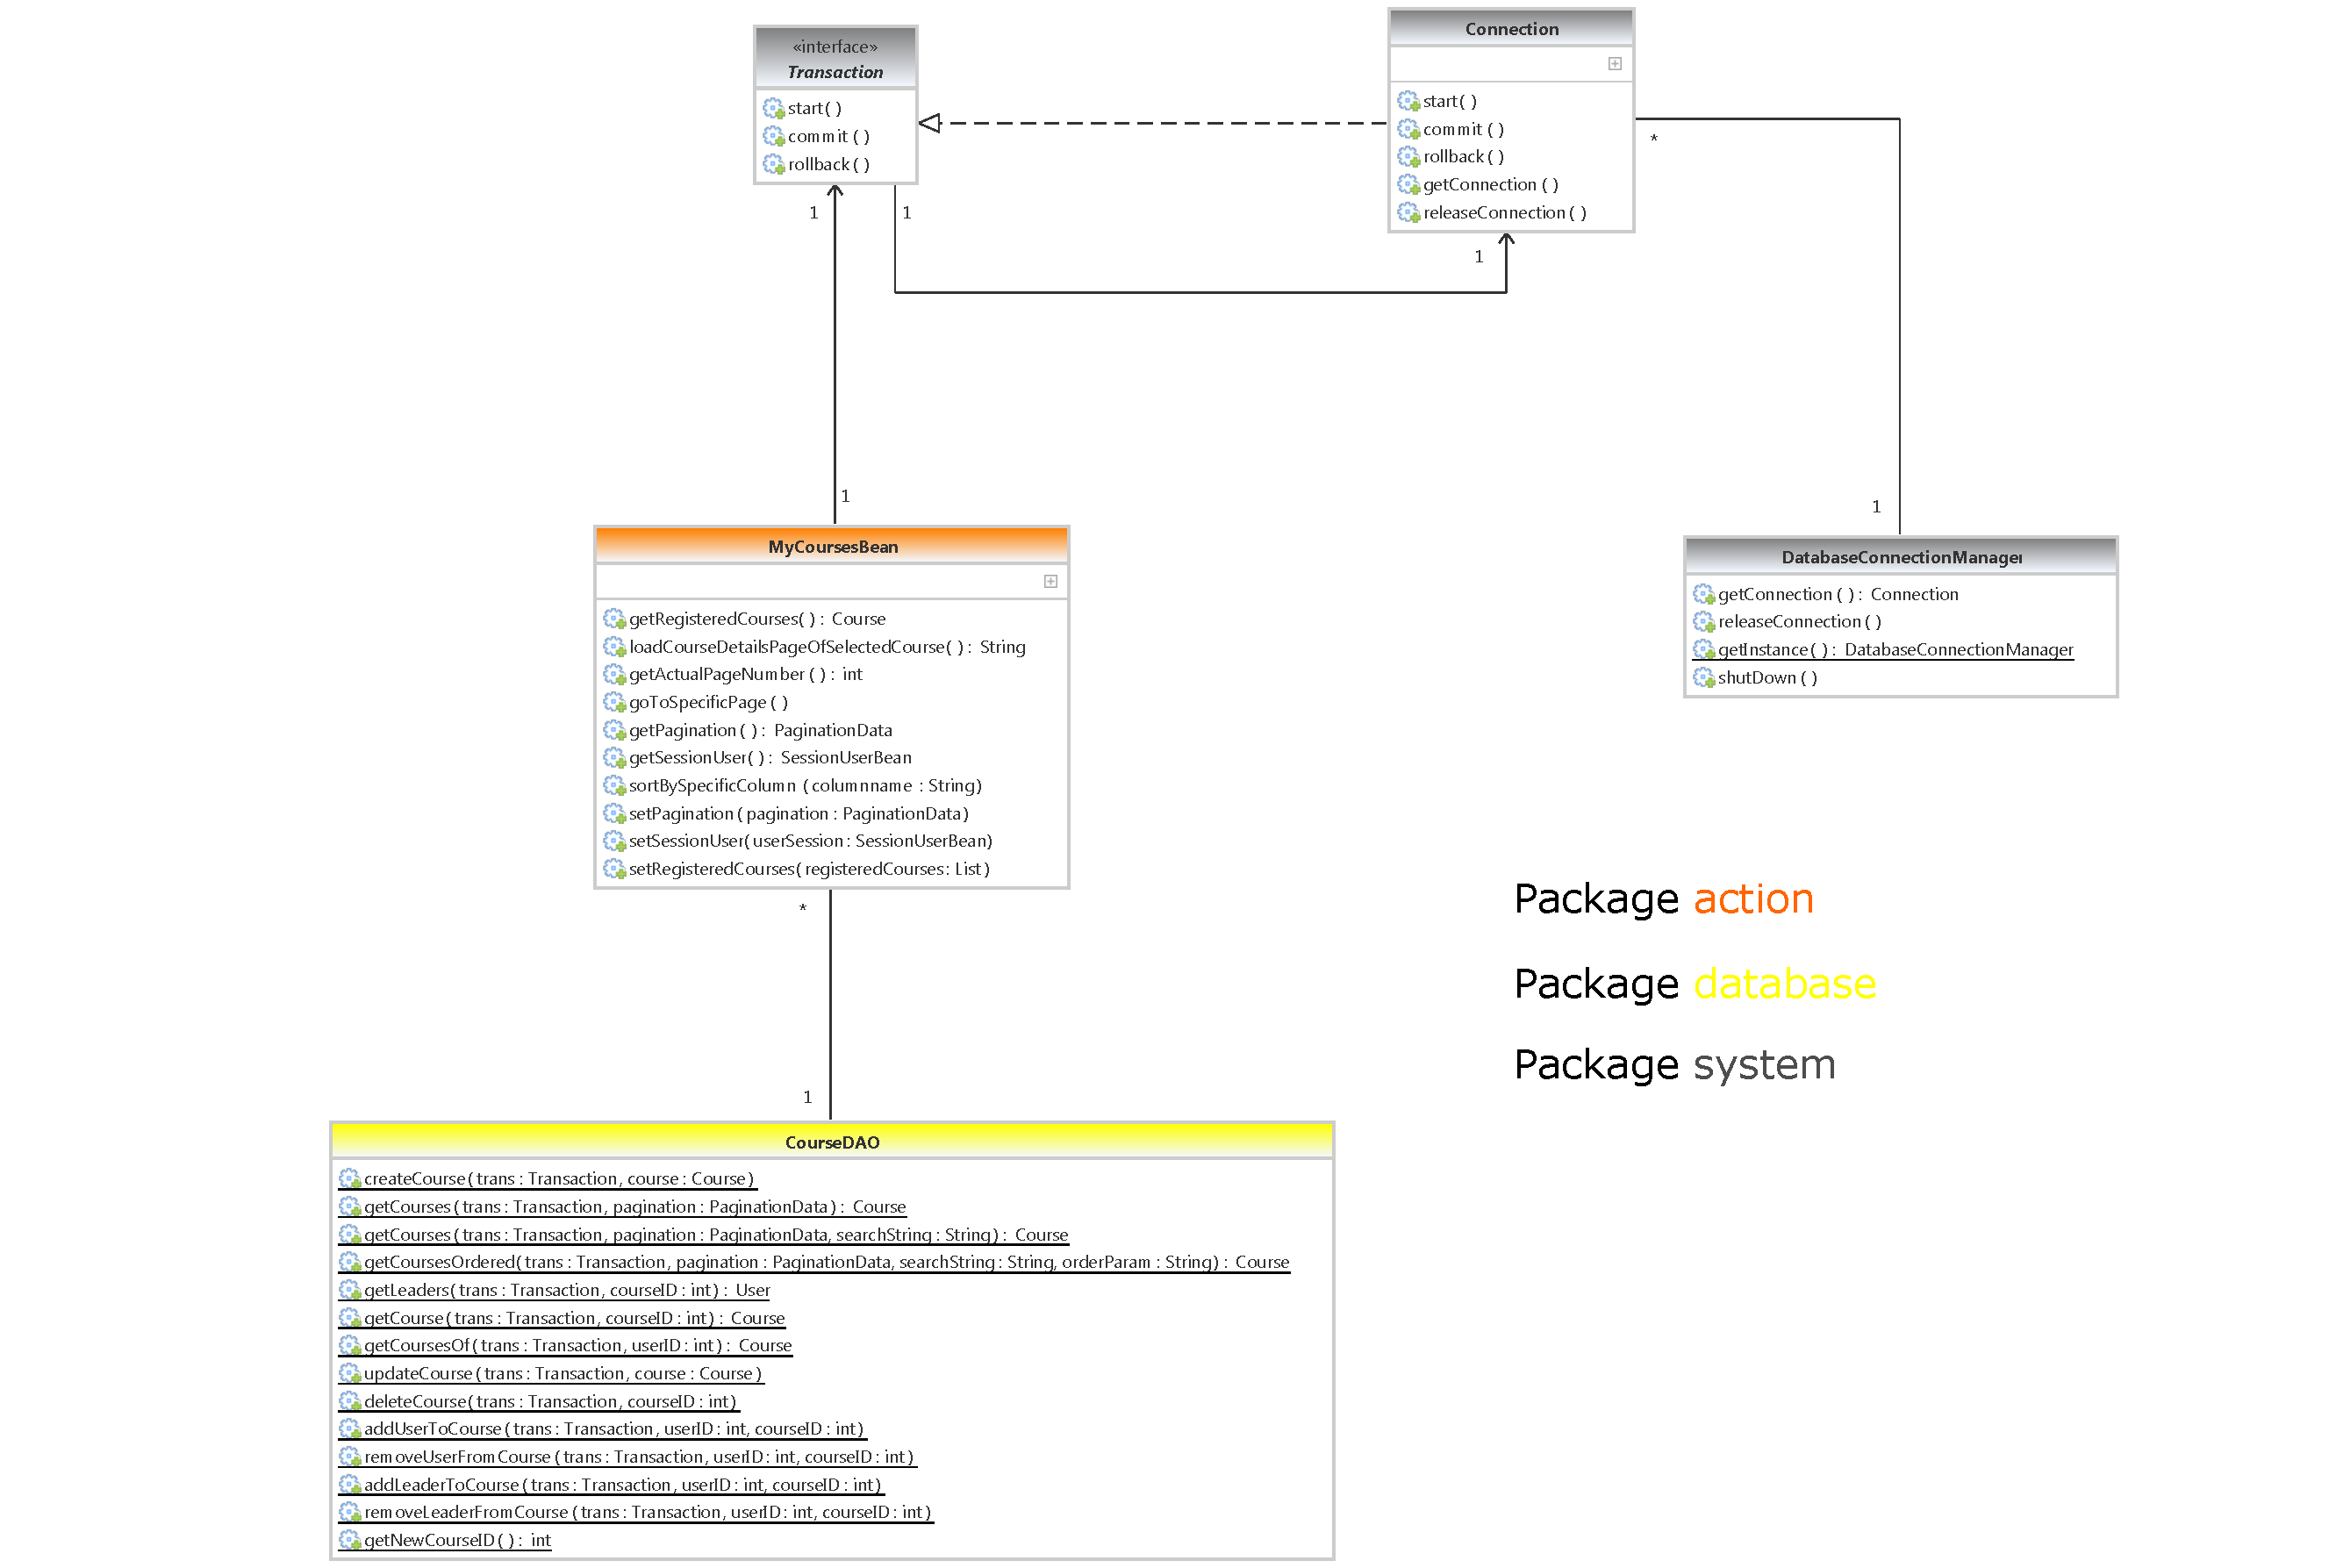
\includegraphics[width=1\linewidth]{Grafiken/Teildiagramm}
	\caption{UML-Teildiagramm zum Interface Transaction}
	\label{fig:Teildiagramm}
	\end{figure}
	\ \\
	In der nachfolgenden Abbildung \ref{fig:UMLKlassendiagrammOhneTransaction_ink} ist das UML-Klassendiagramm des \textbf{ofCourse-Systems} dargestellt.\\
	Um sich dieses Diagramm genauer ansehen zu können, muss es mit einem PDF-Reader
	geöffnet werden, der eine Zoom-Funktion besitzt.
	
	\begin{figure}[h]
	\centering
	\includegraphics[width=1\linewidth, angle=90]{Grafiken/UMLKlassendiagrammOhneTransaction_ink}
	\caption{UML-Klassendiagramm des ofCourse-Systems}
	\label{fig:UMLKlassendiagrammOhneTransaction_ink}
	\end{figure}
	

\chapter{Facelets}

	Dieses Kapitel enthält alle benötigten Facelets, welche die View der Webanwendung darstellen. Jedes Facelet wird in unterschiedliche  Bereiche aufgeteilt:
	\begin{itemize}
		\item \textbf{Beschreibung} Kurzbeschreibung der Funktion/-en des jeweiligen Facelets.
		\item \textbf{Links} enthält alle Links des Facelets, die zu einem anderen Facelet führen.
		\item \textbf{Buttons} listet die sich auf der Seite befindlichen Buttons mit deren hinterlegten Methoden auf.
		\item \textbf{Inputs} enthält eine Liste aller Eingabefelder auf der Seite.
		\item \textbf{Outputs} enthält eine Liste aller Ausgabefelder auf der Seite.
		\item \textbf{Backing Beans} enthält eine Liste aller, mit dem jeweiligen Facelet verbundenen, Beans.
	\end{itemize}
	
	\section{Templates}
		KH, RS
		Das Standard-Template, an dem sich alle Facelets orientieren ist in Abbildung 4.1 zu sehen. Hier wird in drei Teilbereiche unterschieden. Es gibt den Teilbereich \glqq Header\grqq\, welcher hauptsächlich die von der Benutzerrolle abhängige Navigation (\hyperlink{navigation}{navigation.xhtml}) beinhaltet, den Teilbereich \glqq Content\grqq\, welcher abhängig vom jeweils aufgerufenen Facelet befüllt wird und den Teilbereich \glqq Footer\grqq\, welcher den unteren Bereich der dargestellten Seite befüllt (\hyperlink{footer}{footer.xhtml}).

			\begin{figure}[h]
				\centering
				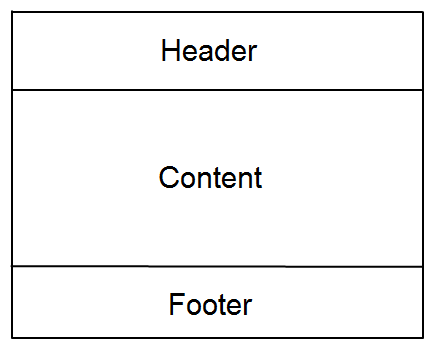
\includegraphics[width=0.3\textwidth]{Grafiken/Template.png}
	  			\caption{Standard-Template für alle Facelets}
			\end{figure}
			
		\paragraph{navigation.xhtml} \hypertarget{navigation}
			RS\\
			\begin{itemize}
				\item \textbf{Beschreibung:} Hier kann, abhängig von der Benutzerrolle, durch die Seite navigiert werden.
				\item \textbf{Links:}
					\begin{itemize}
						\item Suche: Navigiert zur Kurse durchsuchen Seite. \hyperlink{search}{search.xhtml}
						\item Sprache Deutsch: Ändert die angezeigte Sprache zu Deutsch.
						\item Sprache Englisch: Ändert die angezeigte Sprache zu Englisch.
						\item Profil (Benutzer): Navigiert zum eigenen Profil. \hyperlink{profile}{profile.xhtml}
						\item Meine Kurse (Benutzer): Navigiert zur Anzeige der eigenen Kurse. \hyperlink{myCourses}{myCourses.xhtml}
						\item Terminplaner (Benutzer): Navigiert zum persönlichen Terminplaner. \hyperlink{scheduler}{scheduler.xhtml}
						\item Seitenverwaltung (Administrator): Lässt den Seitenadministrator zur Seitenverwaltung navigieren. \hyperlink{adminManagement}{adminManagement.xhtml}
						\item Benutzer aktivieren: (Kursleiter, Administrator): Navigiert zur Benutzer aktivieren Seite. \hyperlink{activateUsers}{activateUsers.xhtml}
					\end{itemize}
				\item \textbf{Buttons:}
					\begin{itemize}
						\item Logout (Benutzer, wenn eingeloggt): Loggt den aktuellen eingeloggten Benutzer aus. \\ Zugehörige Methode: logout()
						\item Anmelden (Anonym): Navigiert zur Registrierungs- und Anmeldeseite. \hyperlink{authenticate}{authenticate.xhtml} \\ Zugehörige Methode: login()
					\end{itemize}
				\item \textbf{Inputs:} -
				\item \textbf{Outputs:}
					\begin{itemize}
						\item Logo: Zeigt verkleinertes, vom Administrator definiertes Logo der Website. Beim klick gelangt der Nutzer zur Startseite \hyperlink{index}{index.xhtml}.
					\end{itemize}
				\item \textbf{BackingBean:}
					\begin{itemize}
						\item Navigation.java
					\end{itemize}
			\end{itemize}

		\paragraph{footer.xhtml} \hypertarget{footer}
			RS\\
			\begin{itemize}
				\item \textbf{Beschreibung:} Dieses Facelet dient der Darstellung des Footers.
				\item \textbf{Links:} -
				\item \textbf{Buttons:}
					\begin{itemize}
						\item AGB: Navigiert zum Facelet mit den Allgemeinen Geschäftsbedingungen, also \hyperlink{agb}{agb.xhtml}. Zugehörige Methode: loadAGBPage()
						\item Impressum: Navigiert zum Facelet mit dem Impressum der Webanwendung, also \hyperlink{imprint}{imprint.xhtml}. Zugehörige Methode: loadImprintPage()
						\item Hilfe: Navigiert zur Hilfeseite, also COMPLETEuserHelp.html. Zugehörige Methode: loadHelpPage()
					\end{itemize}
				\item \textbf{Inputs:} -
				\item \textbf{Outputs:} -
				\item \textbf{BackingBean:}
					\begin{itemize}
						\item Footer.java
					\end{itemize}
			\end{itemize}

		\paragraph{template.xhtml} \hypertarget{template}
			RS\\
			\begin{itemize}
				\item \textbf{Beschreibung:} Dieses Facelet dient der einheitlichen Darstellung und Struktur aller Facelets im System. Letztere ist in Abbildung 4.1 genauer dargestellt.
				\item \textbf{Links:} -
				\item \textbf{Buttons:} -
				\item \textbf{Inputs:}
					\begin{itemize}
						\item Navigation: Bindet \hyperlink{navigation}{navigation.xhtml} in den Header ein.
						\item Footer: Bindet \hyperlink{footer}{footer.xhtml} in den Footer ein.
					\end{itemize}
				\item \textbf{Outputs:} -
				\item \textbf{BackingBean:} -
			\end{itemize}
	
	\section{Facelets}
	
		\subsection{open}
			
			\subsubsection{common}
			
				\paragraph{errorPage.xhtml} \hypertarget{errorPage}
					KH\\
					\begin{itemize}
						\item \textbf{Beschreibung:} Der Benutzer wird auf diese Seite weitergeleitet, wenn Exceptions auftreten, auf die der Nutzer keinen Einfluss hat. Die entsprechende Fehlermeldung wird dann angezeigt.
						\item \textbf{Links:}
						\begin{itemize}
							\item Startseite: Über diesen Link gelangt der Benutzer zurück zur Startseite. (\hyperlink{index}{index.xhtml})
						\end{itemize}
						\item \textbf{Buttons:} -
						\item \textbf{Inputs:} -
						\item \textbf{Outputs:}
						\begin{itemize}
							\item Fehlermeldung: Hier wird die entsprechende Fehlermeldung ausgegeben.
						\end{itemize}
						\item \textbf{BackingBean:} -
					\end{itemize}
			
				\paragraph{index.xhtml} \hypertarget{index}
					RS\\
					\begin{itemize}
						\item \textbf{Beschreibung:} Dieses Facelet stellt die Startseite des Systems dar.
						\item \textbf{Links:}
							\begin{itemize}
								\item Gesamtes Kursangebot, \hyperlink{search}{search.xhtml}
							\end{itemize}
						\item \textbf{Buttons:} -
						\item \textbf{Inputs:} -
						\item \textbf{Outputs:}
							\begin{itemize}
								\item Logo der Website
							\end{itemize}
						\item \textbf{BackingBean:} -
					\end{itemize}
				
				\paragraph{authenticate.xhtml} \hypertarget{authenticate}
				KH\\
				\begin{itemize}
					\item \textbf{Beschreibung:}
					Auf dieser Seite kann man sich im System anmelden, ein neues Benutzerkonto generieren oder ein neues Passwort anfordern.
					\item \textbf{Links:} -
					\item \textbf{Buttons:}
						\begin{itemize}
							\item Registrieren: Durch Drücken dieses Buttons wird der neue Benutzer mit den eingegebenen Daten im System gespeichert und es wird eine Bestätigungsmail mit dem Verifizierungslink an die angegebene E-Mail-Adresse verschickt, sofern alle Daten korrekt eingegeben wurden. \\ Zugehörige Methode: registerUser()
							\item Anmelden: Durch Drücken dieses Buttons wird der registrierte Benutzer im System angemeldet und auf die Seite 'Meine Kurse' (\hyperlink{myCourses}{myCourses.xhtml}) weitergeleitet, sofern Benutzername und Passwort korrekt eingegeben wurden. \\ Zugehörige Methode: login()
							\item Passwort vergessen: Durch Drücken dieses Buttons wird an die angegebene E-Mail-Adresse ein automatisch generiertes Passwort geschickt, sofern die Adresse im System existiert. \\ Zugehörige Methode: resetPassword()
						\end{itemize}
					\item \textbf{Inputs:}
						\begin{itemize}
							\item Anrede (Registrierung): Hier wählt der Benutzer die Anrede 'Herr' oder 'Frau' aus.
							\item Vorname (Registrierung): Hier trägt der Benutzer seinen Vornamen ein.
							\item Name (Registrierung): Hier gibt der Benutzer seinen Namen ein.
							\item Benutzername (Registrierung): Hier gibt der Benutzer einen Benutzernamen ein.
							\item Passwort (Registrierung): Hier trägt der Benutzer ein Passwort ein.
							\item Passwort bestätigen (Registrierung): Hier gibt der Benutzer das gleiche Passwort erneut ein zur Bestätigung.
							\item Geburtstag (Registrierung): Hier gibt der Benutzer sein Geburtsdatum ein.
							\item Straße/Hausnummer (Registrierung): Hier gibt der Benutzer seine Straße und seine Hausnummer ein.
							\item Stadt (Registrierung): Hier trägt der Benutzer seine Stadt ein.
							\item Postleitzahl (Registrierung): Hier trägt der Benutzer seine Postleitzahl ein.
							\item Land (Registrierung): Hier trägt der Benutzer sein Heimatland ein.
							\item E-Mail-Adresse (Registrierung): Hier gibt der Benutzer seine E-Mail-Adresse ein.
							\item AGBs bestätigen (Registrierung): Durch Setzten des Häkchens bestätigt der Benutzer die AGBs. 
							\item Benutzername (Anmeldung): Der Benutzer gibt seinen Benutzernamen ein, mit dem er sich registriert hat.
							\item Passwort (Anmeldung): Der Benutzer gibt sein Passwort ein, mit dem er sich registriert hat.
							\item E-Mail-Adresse (Passwort vergessen): Der Benutzer gibt seine im System bereits gespeicherte E-Mailadresse ein.
						\end{itemize}
					\item \textbf{Outputs:} 
						\begin{itemize}
							\item Vorname Fehlermeldung (Registrierung): Ausgabe der Fehlermeldungen zu den Validatoren des Eingabefeldes.
							\item Name Fehlermeldung (Registrierung): Ausgabe der Fehlermeldungen zu den Validatoren des Eingabefeldes.
							\item Benutzername Fehlermeldung (Registrierung): Ausgabe der Fehlermeldungen zu den Validatoren des Eingabefeldes.
							\item Passwort Fehlermeldung (Registrierung): Ausgabe der Fehlermeldungen zu den Validatoren des Eingabefeldes.
							\item Passwort bestätigen Fehlermeldung (Registrierung): Ausgabe der Fehlermeldungen zu den Validatoren des Eingabefeldes.
							\item Geburtstag Fehlermeldung (Registrierung): Ausgabe der Fehlermeldungen zu den Validatoren des Eingabefeldes.
							\item Straße/Hausnummer Fehlermeldung (Registrierung): Ausgabe der Fehlermeldungen zu den Validatoren des Eingabefeldes.
							\item Stadt Fehlermeldung (Registrierung): Ausgabe der Fehlermeldungen zu den Validatoren des Eingabefeldes.
							\item Postleitzahl Fehlermeldung (Registrierung): Ausgabe der Fehlermeldungen zu den Validatoren des Eingabefeldes.
							\item Land Fehlermeldung (Registrierung): Ausgabe der Fehlermeldungen zu den Validatoren des Eingabefeldes.
							\item E-Mail-Adresse Fehlermeldung (Registrierung): Ausgabe der Fehlermeldungen zu den Validatoren des Eingabefeldes.
							\item AGBs bestätigen Fehlermeldung (Registrierung): Ausgabe der Fehlermeldungen zu den Validatoren des Eingabefeldes.
							\item Benutzername Fehlermeldung (Anmeldung): Ausgabe der Fehlermeldungen zu den Validatoren des Eingabefeldes.
							\item Passwort Fehlermeldung (Anmeldung): Ausgabe der Fehlermeldungen zu den Validatoren des Eingabefeldes.
							\item E-Mail-Adresse Fehlermeldung (Passwort vergessen): Ausgabe der Fehlermeldungen zu den Validatoren des Eingabefeldes.
						\end{itemize}
					\item \textbf{BackingBean:}
						\begin{itemize}
							\item AuthenticateUser.java
							\item RegisterUser.java
							\item LostPassword.java
						\end{itemize}
				\end{itemize}
				
				\paragraph{imprint.xhtml} \hypertarget{imprint}
					KH\\
					\begin{itemize}
						\item \textbf{Beschreibung:} Auf dieser Seite kann das Impressum angezeigt werden.
						\item \textbf{Links:} -
						\item \textbf{Buttons:} -
						\item \textbf{Inputs:} -
						\item \textbf{Outputs:} 
							\begin{itemize}
								\item	Anzeige des Impressums, welches vom Administrator festgelegt wurde.
							\end{itemize}
						\item \textbf{BackingBean:} -
					\end{itemize}
				
				\paragraph{agb.xhtml} \hypertarget{agb}
					RS\\
					\begin{itemize}
						\item \textbf{Beschreibung:} Dieses Facelet dient der Anzeige der Allgemeinen Geschäftsbedingungen.
						\item \textbf{Links:} -
						\item \textbf{Buttons:} -
						\item \textbf{Inputs:} -
						\item \textbf{Outputs:}
							\begin{itemize}
								\item von Betreibern festgelegte Allgemeine Geschäftsbedingungen.
							\end{itemize}
						\item \textbf{BackingBean:} -
					\end{itemize}

		
			\subsubsection{courses}
				
				\paragraph{search.xhtml} \hypertarget{search}
					RS\\
					\begin{itemize}
						\item \textbf{Beschreibung:} Hier können alle Kurse angezeigt und durchsucht werden.
						\item \textbf{Links:} -
						\item \textbf{Buttons:}
							\begin{itemize}
								\item Anzeigen: Zeigt die Angebote im ausgewählten Zeitraum an. \\ Zugehörige Methode: displayCoursesInSpecificPeriod()
								\item Suchen: Durchsucht die Website nach dem eingegebenen Suchbegriff mittels gewählten Suchobjekt. \\ Zugehörige Methode: search()
							\end{itemize}
						\item \textbf{Inputs:}
							\begin{itemize}
								\item Angebotszeitraum: Ermöglicht eine genauere Anzeige des Kursangebots, entweder Tagesangebot, Wochenangebot oder das gesamte Angebot. Die detaillierteren Suchoptionen sind nur für registrierte Benutzer verfügbar.
								\item Suchobjekt (abhängig von Benutzerrolle): Ermöglicht eine genauere Suche, beispielsweise nach Kursen, Kursleitern oder Kurs-ID.
							\end{itemize}
						\item \textbf{Outputs:}
							\begin{itemize}
								\item Tabelle mit Ergebnissen der Suche.
								\item Schaltfläche um zwischen Ergebnissen zu Blättern.
							\end{itemize}
						\item \textbf{BackingBean:}
							\begin{itemize}
								\item SearchCourse.java
							\end{itemize}
					\end{itemize}
				
				\paragraph{courseDetails.xhtml} \hypertarget{courseDetails}
					RS\\
					\begin{itemize}
						\item \textbf{Beschreibung:} Zur genaueren Betrachtung eines einzelnen Kurses wird dieses Facelet benötigt.
						\item \textbf{Links:} -
						\item \textbf{Buttons:}
							\begin{itemize}
								\item Anmelden (Benutzer, noch nicht angemeldet): Meldet den Benutzer zum Kurs an. \\ Zugehörige Methode: signUpForCourse()
								\item Abmelden (Benutzer, wenn angemeldet): Meldet den Benutzer vom Kurs ab. \\ Zugehörige Methode: signOffFromCourse()
								\item Teilnehmer anzeigen (Benutzer): Zeigt die zum Kurs angemeldeten Benutzer an. \hyperlink{listParticipants}{listParticipants.xhtml} \\ Zugehörige Methode: loadParticipantsPage()
								\item Alle auswählen (Benutzer, zum Kurs angemeldet): Wählt alle Kurseinheiten des Kurses aus. \\ Zugehörige Methode: selectAllCourseUnits()
								\item Speichern (Benutzer, zum Kurs angemeldet): Speichert alle ausgewählten Kurseinheiten und meldet den Nutzer dazu an. \\ Zugehörige Methode: signUpForCourseUnits()
								\item Bearbeiten (Administrator, noch nicht im Bearbeitungsmodus): Ermöglicht die Bearbeitung der einzelnen Kursdetails. \\ Zugehörige Methode: editCourse()
								\item Speichern (Administrator, im Bearbeitungsmodus): Speichert alle vorgenommenen Kursänderungen. \\ Zugehörige Methode: saveCourse()
								\item Hinzufügen (Administrator): Fügt einen Kursleiter zum Kurs hinzu. Zugehörige Methode: addCourseLeader()
								\item Kurseinheit anlegen (Kursleiter): Erstellt eine neue Kurseinheit zum Kurs. \hyperlink{editCourseUnit}{editCourseUnit.xhtml} \\ Zugehörige Methode: loadCreateCourseUnitPage()
								\item Kurseinheit bearbeiten (Kursleiter): Ermöglicht die Bearbeitung einer einzelnen Kurseinheit. \hyperlink{editCourseUnit}{editCourseUnit.xhtml} \\ Zugehörige Methode: loadEditCourseUnitPage()
								\item Kurs löschen (Administrator): Löscht den Kurs. \\ Zugehörige Methode: deleteCourse()
							\end{itemize}
						\item \textbf{Inputs:}
							\begin{itemize}
								\item Kursnews erhalten: Trägt Benutzer bei Anmeldung zum Kurs in die Kursnews ein.
								\item Kurseinheit auswählen: Wählt Kurseinheit aus, zu der sich der Nutzer anmelden möchte.
								\item Kursleiter auswählen (Administrator): Wählt Kursleiter aus, welcher gelöscht werden soll.
								\item Kursleiter Name (Administrator): Eingabefeld für den Namen eines neuen Kursleiters.
								\item Kursleiter E-Mail (Administrator): Eingabefeld für die E-Mail Adresse eines neuen Kursleiters.
								\item Kursbeschreibung (Administrator): Eingabefeld für die Kursbeschreibung.
								\item Minimale Teilnehmerzahl (Administrator): Eingabefeld für die minimale Teilnehmerzahl des Kurses.
								\item Maximale Teilnehmerzahl (Administrator): Eingabefeld für die maximale Teilnehmerzahl des Kurses.
								\item Startdatum (Administrator): Eingabefeld für das Startdatum des Kurses.
								\item Enddatum (Administrator): Eingabefeld für das Enddatum des Kurses.
							\end{itemize}
						\item \textbf{Outputs:}
							\begin{itemize}
								\item Tabelle Kursleiter: Tabelle mit den Kontaktinformationen der/des Kursleiters.
								\item Tabelle Kurseinheiten: Tabelle mit allen Kurseinheiten des Kurses und zugehörigen Informationen wie Ort, Preis oder Datum.
								\item Kurs-ID: Zeigt die zum Kurs zugehörige ID an.
								\item Kursbeschreibung: Zeigt die Beschreibung zum Kurs an.
								\item Minimale Teilnehmerzahl: Zeigt die für den Kurs minimale Teilnehmerzahl an.
								\item Maximale Teilnehmerzahl: Zeigt die für den Kurs maximale Teilnehmerzahl an.
								\item Fehlermeldung zu den einzelnen Eingabefeldern, bei falscher Eingabe.
							\end{itemize}
						\item \textbf{BackingBean:}
							\begin{itemize}
								\item CourseDetail.java
								\item CourseManagement.java
							\end{itemize}
					\end{itemize}
		
		\subsection{users}
		
			\subsubsection{registeredUser}
				
				\paragraph{myCourses.xhtml} \hypertarget{myCourses}
					KH\\
					\begin{itemize}
						\item \textbf{Beschreibung:} Auf dieser Seite werden alle Kurse angezeigt, in die der Teilnehmer eingetragen ist.
						\item \textbf{Links:}
							\begin{itemize}
								\item Kurstitel: Über die Kurstitel gelangt der Benutzer auf die jeweilige Kursdetailseite. (\hyperlink{courseDetails}{courseDetails.xhtml})
							\end{itemize}
						\item \textbf{Buttons:} -
						\item \textbf{Inputs:} -
						\item \textbf{Outputs:}
							\begin{itemize}
								\item Tabelle Auflistung aller Kurse: Hier werden dem Benutzer alle seine angemeldeten Kurse angezeigt.
							\end{itemize}
						\item \textbf{BackingBean:}
							\begin{itemize}
								\item MyCourses.java
							\end{itemize}
					\end{itemize}
				
				\paragraph{profile.xhtml} \hypertarget{profile}
					KH\\
					\begin{itemize}
						\item \textbf{Beschreibung:} Auf dieser Seite werden die persönlichen Daten und der Kontostand des Benutzers angezeigt. Der Benutzer kann die Daten ändern und sein Konto aufladen. Der Kursleiter kann hier den Benutzer aktivieren, und der Administrator den Benutzer löschen.
						\item \textbf{Links:} -
						\item \textbf{Buttons:}
							\begin{itemize}
								\item Bearbeiten: Nach Klicken auf diesen Button können die persönlichen Daten geändert werden. Der Button trägt nun die Aufschrift 'Speichern' und ist mit dessen dazugehöriger Methode hinterlegt. \\ Zugehörige Methode: editUserData()
								\item Speichern: Durch Drücken dieses Buttons werden die vorgenommenen Änderungen gespeichert, sofern alle Daten korrekt eingegeben wurden. Bei Änderung der E-Mail-Adresse wird außerdem eine Bestätigungsmail mit einem Verifizierungslink verschickt. Bei erfolgreicher Speicherung erscheint der Button 'Bearbeiten' anstelle des Button 'Speichern'. \\ Zugehörige Methode: saveUserData()
								\item Durchsuchen: Durch Drücken dieses Buttons kann das eigene Dateiverzeichnis nach einem Bild durchsucht werden.
								\item Hochladen: Durch Drücken dieses Buttons wird das ausgewählte Profilbild hochgeladen. \\ Zugehörige Methode: uploadProfilPic()
								\item Konto aufladen: Durch Klicken dieses Buttons wird der Benutzer auf die Seite 'Kontoaufladung' (\hyperlink{buyCredits}{buyCredits.xhtml})  weitergeleitet. \\ Zugehörige Methode: depositMoneyPerCreditCard()
								\item Benutzer löschen: Durch Drücken dieses Buttons entfernt der Administrator diesen Benutzer aus dem System, oder der Benutzer kann sich selbst auf inaktiv setzen. \\ Zugehörige Methoden: deleteUser(), setUserInactive() 
							\end{itemize}
						\item \textbf{Inputs:}
							\begin{itemize}
								\item Vorname: Hier kann der Benutzer seinen Vornamen ändern.
								\item Name: Hier kann der Benutzer seinen Namen ändern.
								\item Geburtstag: Hier kann der Benutzer sein Geburtsdatum ändern.
								\item Straße/Hausnummer: Hier kann der Benutzer seine Straße und Hausnummer ändern.
								\item Stadt: Hier kann der Benutzer seine Stadt ändern.
								\item Postleitzahl: Hier kann der Benutzer seine Postleitzahl ändern.
								\item Land: Hier kann der Benutzer seine Land ändern.
								\item E-Mail-Adresse: Hier kann der Benutzer seine E-Mail-Adresse ändern.
								\item Benutzername: Hier kann der Benutzer seinen Benutzernamen ändern.
								\item Passwort: Hier kann der Benutzer sein Passwort ändern.
								\item Passwort bestätigen: Hier muss der Benutzer sein geändertes Passwort bestätigen.
								\item Benutzerrolle: Hier kann der Administrator die Benutzerrolle eines Nutzers ändern.
								\item Profilbild: Hier kann der Benutzer sein Profilbild ändern.
							\end{itemize}
						\item \textbf{Outputs:}
							\begin{itemize}
								\item Benutzer-ID: Ausgabe der automatisch generierten ID.
								\item Vorname Fehlermeldung: Ausgabe der Fehlermeldungen zu den Validatoren des Eingabefeldes.
								\item Name Fehlermeldung: Ausgabe der Fehlermeldungen zu den Validatoren des Eingabefeldes.
								\item Geburtstag Fehlermeldung: Ausgabe der Fehlermeldungen zu den Validatoren des Eingabefeldes.
								\item Straße/Hausnummer Fehlermeldung: Ausgabe der Fehlermeldungen zu den Validatoren des Eingabefeldes.
								\item Stadt Fehlermeldung: Ausgabe der Fehlermeldungen zu den Validatoren des Eingabefeldes.
								\item Postleitzahl Fehlermeldung: Ausgabe der Fehlermeldungen zu den Validatoren des Eingabefeldes.
								\item Land Fehlermeldung: Ausgabe der Fehlermeldungen zu den Validatoren des Eingabefeldes.
								\item E-Mail-Adresse Fehlermeldung: Ausgabe der Fehlermeldungen zu den Validatoren des Eingabefeldes.
								\item Benutzername Fehlermeldung: Ausgabe der Fehlermeldungen zu den Validatoren des Eingabefeldes.
								\item Passwort Fehlermeldung: Ausgabe der Fehlermeldungen zu den Validatoren des Eingabefeldes.
								\item Passwort bestätigen Fehlermeldung: Ausgabe der Fehlermeldungen zu den Validatoren des Eingabefeldes.
								\item Profilbild Fehlermeldung: Ausgabe der Fehlermeldungen zu den Validatoren des Eingabefeldes.
								\item Kontostand: Ausgabe des aktuellen Kontostandes.
								\item Tabelle Auflistung der Trainingskurse: Hier werden dem Kursleiter alle Kurse aufgelistet, die er leitet.
							\end{itemize}
						\item \textbf{BackingBean:}
							\begin{itemize}
								\item UserProfile.java
								\item UserManagement.java				
							\end{itemize}
					\end{itemize}
				
				\paragraph{buyCredits.xhtml} \hypertarget{buyCredits}
					RS\\
					\begin{itemize}
						\item \textbf{Beschreibung:} Hier kann der Nutzer mittels Kreditkarte seinen systeminternen Kontostand erhöhen.
						\item \textbf{Links:} -
						\item \textbf{Buttons:}
							\begin{itemize}
								\item Konto aufladen: Führt die Kontoaufladung aus. \\ Zugehörige Methode: depositAmount()
							\end{itemize}
						\item \textbf{Inputs:}
							\begin{itemize}
								\item CVC-Nummer: Prüfnummer der Kreditkarte.
								\item Ablaufdatum: Ablaufdatum der Kreditkarte.
								\item Nachname: Nachname des Nutzers zur Kontoaufladung.
								\item Vorname: Vorname des Nutzers zur Kontoaufladung.
								\item Kreditinstitut: Name des Kreditinstitutes des Nutzers zur Kontoaufladung.
								\item Kreditkartennummer: Nummer der Kreditkarte des Nutzers zur Kontoaufladung.
								\item Betrag: Geldbetrag, welcher auf das systeminterne Konto des Nutzers gebucht werden soll.
							\end{itemize}
						\item \textbf{Outputs:}
							\begin{itemize}
								\item Fehlermeldung zu den einzelnen Eingabefeldern, bei falscher Eingabe.
								\item Bestätigungsmeldung bei erfolgreicher Aufladung des Kontos.
							\end{itemize}
						\item \textbf{BackingBean:}
							\begin{itemize}
								\item PayementOnline.java
							\end{itemize}
					\end{itemize}
				
				\paragraph{scheduler.xhtml} \hypertarget{scheduler}
					RS\\
					\begin{itemize}
						\item \textbf{Beschreibung:} Persönlicher Terminplaner mit anstehenden Kursen.
						\item \textbf{Links:}
							\begin{itemize}
								\item Wochenansicht vorwärts: Zeigt die Termine der nächsten Woche an.
								\item Wochenansicht rückwärts: Zeigt die Termine der letzten Woche an.
							\end{itemize}
						\item \textbf{Buttons:} -
						\item \textbf{Inputs:} -
						\item \textbf{Outputs:}
							\begin{itemize}
								\item Wochentabelle: Zeigt von Montag bis Sonntag alle belegten Kurseinheiten an. Orientiert sich am klassischen Stundenplan, also mit stündlicher Ansicht.
							\end{itemize}
						\item \textbf{BackingBean:}
							\begin{itemize}
								\item Scheduler.java
							\end{itemize}
					\end{itemize}
				
				\paragraph{leaderProfile.xhtml} \hypertarget{leaderProfile}
					KH\\
					\begin{itemize}
						\item \textbf{Beschreibung:} Auf dieser Seite werden die Daten des Kursleiters, mit Ausnahme von sensiblen Daten wie Passwort oder Kontostand, und die von ihm geleiteten Kurse angezeigt.
						\item \textbf{Links:} -
						\item \textbf{Buttons:} -
						\item \textbf{Inputs:} -
						\item \textbf{Outputs:} 
							\begin{itemize}
								\item Tabelle Auflistung Kursleiterdaten: Hier werden die Daten des Kursleiters und die von ihm geleiteten Kurse angezeigt.
							\end{itemize}
						\item \textbf{BackingBean:}
						\begin{itemize}
							\item UserProfile.java			
						\end{itemize}
					\end{itemize}
				
				\paragraph{listParticipants.xhtml} \hypertarget{listParticipants}
					KH\\
					\begin{itemize}
						\item \textbf{Beschreibung:} Hier kann der registrierte Benutzer die Teilnehmer eines Kurses mit Benutzername und Profilbild ansehen. Dem Kursleiter werden zusätzlich die E-Mail-Adresse und die Information über den Erhalt von Kursnews angezeigt. Außerdem kann er einen Teilnehmer aus dem Kurs entfernen.
						\item \textbf{Links:} -
						\item \textbf{Buttons:}
							\begin{itemize}
								\item Löschen: Durch Drücken dieses Buttons kann der Kursleiter den entsprechenden Benutzer aus dem Kurs entfernen. \\ Zugehörige Methode: deleteUserFromCourse()
							\end{itemize}
						\item \textbf{Inputs:}
							 \begin{itemize}
							 	\item Entfernen: Durch Setzen des Häkchens wählt der Kursleiter diesen Benutzer aus, um ihn anschließend über den Button 'Löschen' zu entfernen.
							 \end{itemize}
						\item \textbf{Outputs:} 
							\begin{itemize}
								\item Tabelle Auflistung Kursteilnehmer: Hier werden die Teilnehmer des Kurses angezeigt.
							\end{itemize}
						\item \textbf{BackingBean:}
							\begin{itemize}
								\item ListParticipants.java
							\end{itemize}
					\end{itemize}
			
			\subsubsection{courseLeader}
			
				\paragraph{editCourseUnit.xhtml} \hypertarget{editCourseUnit}
					KH\\
					\begin{itemize}
						\item \textbf{Beschreibung:} Auf dieser Seite können Kursleiter beziehungsweise Administratoren Kurseinheiten anlegen und bearbeiten, oder Kursteilnehmer hinzufügen und entfernen
						\item \textbf{Links:} -
						\item \textbf{Buttons:}
							\begin{itemize}
								\item Bearbeiten (Kurseinheit): Nach Klicken auf diesen Button können die Daten der Kurseinheit geändert beziehungsweise eingetragen werden. Der Button trägt nun die Aufschrift 'Speichern' und ist mit dessen dazugehöriger Methode hinterlegt. \\ Zugehörige Methode: editCourseUnit()
								\item Speichern (Kurseinheit): Durch Drücken dieses Buttons werden die vorgenommenen Änderungen gespeichert, sofern alle Daten korrekt eingegeben wurden. Bei erfolgreicher Speicherung erscheint der Button 'Bearbeiten' anstelle des Button 'Speichern'. \\ Zugehörige Methode: saveCourseUnit()
								\item Löschen (Kurseinheit): Durch Drücken des Button 'Löschen' wird die Kurseinheit entfernt. \\ Zugehörige Methode: deleteCourseUnit()
								\item Löschen (Teilnehmer): Durch Drücken dieses Buttons wird der markierte Teilnehmer aus der Kurseinheit entfernt. \\ Zugehörige Methode: deleteUserFromCourseUnit()
								\item Hinzufügen (Teilnehmer): Durch Drücken dieses Buttons wird der angegebene Teilnehmer zu dieser Kurseinheit hinzugefügt, sofern der Benutzername im System existiert und die Daten korrekt eingegeben wurden. \\ Zugehörige Methode: addUserToCourseUnit()
							\end{itemize}
						\item \textbf{Inputs:}
							\begin{itemize}
								\item Termin: Hier gibt der Kursleiter den Termin der Kurseinheit ein.
								\item Straße/ Hausnummer: Hier gibt der Kursleiter Straße und Hausnummer ein.
								\item Postleitzahl: Hier gibt der Kursleiter die entsprechende Postleitzahl ein.
								\item Stadt: Hier gibt der Kursleiter die Stadt ein, in der die Kurseinheit stattfindet.
								\item Ort: Hier gibt der Kursleiter den Ort (Raumnummer, Turnhalle,..) ein, in dem die Kurseinheit stattfindet.
								\item Beschreibung: Hier gibt der Kursleiter die Beschreibung der Kurseinheit ein.
								\item Preis: Hier gibt der Kursleiter den Preis der Kurseinheit ein.
								\item Kursleiter: Hier wird der Leiter des Kurses angezeigt.
								\item Mindestteilnehmerzahl: Hier gibt der Kursleiter die minimale Teilnehmerzahl der Kurseinheit an.
								\item Maximale Teilnehmerzahl: Hier gibt der Kursleiter die maximale Teilnehmerzahl der Kurseinheit an.
								\item Teilnehmer markieren: Hier kann der Kursleiter einen Hacken setzen, um den Teilnehmer für das anschließende Löschen zu markieren.
								\item Benutzer-ID: Hier gibt der Kursleiter die Benutzer-ID des Teilnehmers an, welchen er zu der Kurseinheit hinzufügen will.
								\item Name (Teilnehmer): Hier gibt der Kursleiter den entsprechenden Namen des Teilnehmers an, welchen er zu der Kurseinheit hinzufügen will.
								\item Vorname (Teilnehmer): Hier gibt der Kursleiter den entsprechenden Vornamen des Teilnehmers an, welchen er zu der Kurseinheit hinzufügen will.
								\item Checkbox regelmäßig: Durch Setzen dieses Hackens markiert der Kursleiter den Kurs als regelmäßig.
								\item Turnus: Hier wählt der Kursleiter aus einem Drop-Down Menü aus, ob der Kurs beispielsweise wöchentlich stattfinden soll.
								\item Einheitenanzahl: Hier gibt der Kursleiter an, wie viele Einheiten er anlegen will.
							\end{itemize}
						\item \textbf{Outputs:}
							\begin{itemize}
								\item Termin (Fehlermeldung): Ausgabe der Fehlermeldungen zu den Validatoren des Eingabefeldes.
								\item Straße/ Hausnummer (Fehlermeldung): Ausgabe der Fehlermeldungen zu den Validatoren des Eingabefeldes.
								\item Postleitzahl (Fehlermeldung): Ausgabe der Fehlermeldungen zu den Validatoren des Eingabefeldes.
								\item Stadt (Fehlermeldung): Ausgabe der Fehlermeldungen zu den Validatoren des Eingabefeldes.
								\item Raum (Fehlermeldung): Ausgabe der Fehlermeldungen zu den Validatoren des Eingabefeldes.
								\item Beschreibung (Fehlermeldung): Ausgabe der Fehlermeldungen zu den Validatoren des Eingabefeldes.
								\item Preis (Fehlermeldung): Ausgabe der Fehlermeldungen zu den Validatoren des Eingabefeldes.
								\item Kursleiter (Fehlermeldung): Ausgabe der Fehlermeldungen zu den Validatoren des Eingabefeldes.
								\item Mindestteilnehmerzahl (Fehlermeldung): Ausgabe der Fehlermeldungen zu den Validatoren des Eingabefeldes.
								\item Maximale Teilnehmerzahl (Fehlermeldung): Ausgabe der Fehlermeldungen zu den Validatoren des Eingabefeldes.
								\item Status: Hier wird ausgegeben, wie viele Teilnehmer bereits in der Kurseinheit eingetragen sind.
								\item Benutzer-ID (Fehlermeldung): Ausgabe der Fehlermeldungen zu den Validatoren des Eingabefeldes.
								\item Name (Teilnehmer (Fehlermeldung)): Ausgabe der Fehlermeldungen zu den Validatoren des Eingabefeldes.
								\item Vorname (Teilnehmer (Fehlermeldung)): Ausgabe der Fehlermeldungen zu den Validatoren des Eingabefeldes.
								\item Einheitenanzahl: Ausgabe der Fehlermeldungen zu den Validatoren des Eingabefeldes.
							\end{itemize}
						\item \textbf{BackingBean:}
							\begin{itemize}
								\item CourseUnitManagement.java
							\end{itemize}
					\end{itemize}
				
				\paragraph{activateUsers.xhtml} \hypertarget{activateUsers}
					KH\\
					\begin{itemize}
						\item \textbf{Beschreibung:} Hier werden alle im System noch nicht aktivierten Benutzer angezeigt. Diese können nun vom Kursleiter oder Administrator aktiviert werden. 
						\item \textbf{Links:} -
						\item \textbf{Buttons:}
							\begin{itemize}
								\item Benutzer aktivieren: Durch Klicken dieses Buttons wird der Account des markierten Benutzers aktiviert. \\ Zugehörige Methode: activateAccounts()
							\end{itemize}
						\item \textbf{Inputs:}
							\begin{itemize}
								\item Benutzer aktivieren: Der Kursleiter kann durch Setzen des Häkchens Benutzer auswählen, um diese anschließend zu aktivieren.
							\end{itemize}
						\item \textbf{Outputs:}
							\begin{itemize}
								\item Tabelle Auflistung Benutzerdaten: Hier werden ausgewählte Daten aller im System registrierten, aber noch nicht aktivierten Benutzer angezeigt.
							\end{itemize}
						\item \textbf{BackingBean:}
							\begin{itemize}
								\item AccountManagement.java
							\end{itemize}
					\end{itemize}
			
			\subsubsection{systemAdministrator}
			
				\paragraph{adminManagement.xhtml} \hypertarget{adminManagement}
					RS\\
					\begin{itemize}
						\item \textbf{Beschreibung:} Dieses Facelet stellt die zentrale Systemverwaltung für den Administrator dar. Hier kann er Kurse und Benutzer jeweils anlegen und verwalten, das Konto eines Nutzers aufladen, zu den Statistiken gelangen, den Überziehungskredit für Nutzer festlegen und das System optisch anpassen.
						\item \textbf{Links:} -
						\item \textbf{Buttons:}
							\begin{itemize}
								\item Benutzer verwalten: Navigiert zu Benutzer verwalten Seite. \hyperlink{listUsers}{listUsers.xhtml} \\ Zugehörige Methode: loadManageUserPage()
								\item Benutzer anlegen: Navigiert zu Benutzer anlegen Seite. \hyperlink{createUser}{createUser.xhtml} \\ Zugehörige Methode: loadCreateNewUserPage()
								\item Kurse verwalten: Navigiert zu Kurse verwalten Seite. \hyperlink{search}{search.xhtml}\\ Zugehörige Methode: loadManageCoursesPage()
								\item Kurs anlegen: Navigiert zu Kurs anlegen Seite. \hyperlink{createCourse}{createCourse.xhtml} \\ Zugehörige Methode: loadCreateNewCoursePage()
								\item Aktivierungsmodalität speichern: Speichert die ausgewählte Art der Benutzeraktivierung. \\ Zugehörige Methode: determineAccountActivationType()
								\item Guthaben aufladen: Erhöht den Kontostand eines bestimmten Benutzer um die eingegebene Summe. \\ Zugehörige Methode: depositAmountOnUserAccount()
								\item Überziehungswert speichern: Speichert den Wert der möglichen Kontoüberziehung. \\ Zugehörige Methode: determineOverdraftCredit()
								\item Statistiken anzeigen: Navigiert zur Anwendungsstatistik Seite. \hyperlink{statistics}{statistics.xhtml} \\ Zugehörige Methode: loadStatisticPage()
								\item Logo durchsuchen: Öffnet ein Fenster um das Logo der Website vom Computer auszuwählen.
								\item Logo speichern: Speichert das benutzerdefinierte Logo für die Website. \\ Zugehörige Methode: uploadLogo()
								\item Oberfläche CSS durchsuchen: Öffnet ein Fenster um die benutzerdefinierte CSS-Datei vom Computer auszuwählen. 
								\item Oberfläche CSS speichern: Speichert die benutzerdefinierte CSS-Datei. \\ Zugehörige Methode: uploadCustomStyleCSS()
								\item Impressum bearbeiten: Navigiert zur Impressum bearbeiten Seite. \hyperlink{editImprint}{editImprint.xhtml} \\ Zugehörige Methode: loadEditImprintPage()
							\end{itemize}
						\item \textbf{Inputs:}
							\begin{itemize}
								\item Accountaktivierung: Auswahlfeld um Registrierungsmodalität festzulegen.
								\item Benutzer-ID: ID des Benutzers, dessen Kontostand erhöht werden soll.
								\item Benutzername: Name des Benutzers, dessen Kontostand erhöht werden soll.
								\item Betrag: Betrag, welcher dem Nutzer gutgeschrieben werden soll.
								\item Überziehungswert: Betrag, welcher im ganzen System zur Überziehung des Kontos akzeptiert wird.
							\end{itemize}
						\item \textbf{Outputs:}
							\begin{itemize}
								\item Fehlermeldung zu den einzelnen Eingabefeldern, bei falscher Eingabe oder fehlerhaften Uploads.
							\end{itemize}
						\item \textbf{BackingBean:}
							\begin{itemize}
								\item SystemConfiguration.java
								\item PaymentOffline.java
							\end{itemize}
					\end{itemize}
											
				\paragraph{listUsers.xhtml} \hypertarget{listUsers}
					KH\\
					\begin{itemize}
						\item \textbf{Beschreibung:} Hier werden alle im System registrierten Benutzer angezeigt. Einzelne Benutzer können vom Administrator nach verschiedenen Kriterien gefiltert werden. 
						\item \textbf{Links:} -
						\item \textbf{Buttons:}
						\begin{itemize}
							\item Suchen: Durch Drücken dieses Buttons werden die Benutzer nach den eingegebenen Kriterien durchsucht und in der Liste angezeigt. \\ Zugehörige Methode: search()
						\end{itemize}
						\item \textbf{Inputs:}
						\begin{itemize}
							\item Kriterienauswahl: Hier kann der Kursleiter auswählen, ob er nach 'Benutzer-ID', 'Benutzername', 'Name' oder 'Benutzerrolle' suchen will.
							\item Suchbegriff: Hier gibt der Kursleiter den entsprechenden Suchbegriff ein.
						\end{itemize}
						\item \textbf{Outputs:}
						\begin{itemize}
							\item Tabelle Auflistung Benutzerdaten: Hier werden ausgewählte Daten aller im System registrierten Benutzer angezeigt.
							\item Suchbegriff (Fehlermeldung): Ausgabe der Fehlermeldungen zu den Validatoren des Eingabefeldes.
						\end{itemize}
						\item \textbf{BackingBean:}
						\begin{itemize}
							\item SearchUser.java
						\end{itemize}
					\end{itemize}
				
				\paragraph{createUser.xhtml} \hypertarget{createUser}
					RS\\
					\begin{itemize}
						\item \textbf{Beschreibung:} Hier kann der Systemadministrator einen neuen Benutzer mit festgelegter Benutzerrolle anlegen.
						\item \textbf{Links:} -
						\item \textbf{Buttons:}
							\begin{itemize}
								\item Durchsuchen: Öffnet ein Fenster um auf dem Computer nach einem Profilbild zu suchen. 
								\item Hochladen: Lädt das ausgewählte Profilbild hoch.\\ Zugehörige Methode: uploadprofilePic()
								\item Benutzer anlegen: Legt den Benutzer an. \\ Zugehörige Methode: createUser()
							\end{itemize}
						\item \textbf{Inputs:}
							\begin{itemize}
								\item Anrede: Herr oder Frau.
								\item Vorname: Vorname des neuen Benutzers.
								\item Nachname: Nachname des neuen Benutzers.
								\item Geburtsdatum: Geburtsdatum des neuen Benutzers.
								\item Straße: Straße des neuen Benutzers.
								\item Postleitzahl: Postleitzahl des neuen Benutzers.
								\item Stadt: Stadt des neuen Benutzers.
								\item Benutzername: Benutzername des neuen Benutzers.
								\item Passwort: Passwort des neuen Benutzers.
								\item Passwort wiederholen: Passwortfeld um Passwort sicherzustellen.
								\item E-Mail: E-Mail Adresse des neuen Benutzers.
								\item Benutzerrolle: Benutzerrolle des neuen Benutzers, Administrator, Kursleiter oder normaler Benutzer.
							\end{itemize}
						\item \textbf{Outputs:}
							\begin{itemize}
								\item Fehlermeldung zu den einzelnen Eingabefeldern, bei falscher Eingabe.
								\item Benutzer-ID: ID des neuen Benutzers.
								\item Profilbild: Dummy-Profilbild des neuen Benutzers.
							\end{itemize}
						\item \textbf{BackingBean:}
							\begin{itemize}
								\item UserManagement.java
							\end{itemize}
					\end{itemize}
				
				\paragraph{createCourse.xhtml} \hypertarget{createCourse}
					KH\\
					\begin{itemize}
						\item \textbf{Beschreibung:} Hier kann der Administrator einen neuen Kurs anlegen, einen bestehenden Kurs löschen, oder Kursleiter zu bestehenden Kursen hinzufügen. Der Kursleiter kann außerdem Kurseinheiten erstellen.
						\item \textbf{Links:} -
						\item \textbf{Buttons:}
							\begin{itemize}
								\item Kurs anlegen:  Durch Drücken dieses Buttons wird der Kurs angelegt, sofern alle Daten korrekt eingegeben wurden. \\ Zugehörige Methode: createCourse()
								\item Löschen (Kursleiter): Durch Drücken dieses Buttons löscht der Administrator den ausgewählten Kursleiter aus diesem Kurs. \\ Zugehörige Methode: removeCourseLeader()
								\item Hinzufügen (Kursleiter): Durch Drücken dieses Buttons wird der angegebene Kursleiter zum Kurs hinzugefügt, sofern alle Eingabe korrekt waren.	\\ Zugehörige Methode: addCourseLeader()
							\end{itemize}
						\item \textbf{Inputs:}
							\begin{itemize}
								\item Kursname: Hier gibt der Administrator den Kursnamen ein.
								\item Beschreibung: Hier gibt der Administrator die Beschreibung des Kurses ein.
								\item Maximale Teilnehmerzahl: Hier gibt der Administrator die maximale Teilnehmerzahl des Kurses an.
								\item Startdatum: Hier trägt der Administrator das Startdatum des Kurses ein.
								\item Enddatum: Hier trägt der Administrator das Enddatum des Kurses ein.
								\item Name (Kursleiter): Hier gibt der Administrator den Namen des Kursleiters ein, den er zum Kurs hinzufügen will.
								\item E-Mail-Adresse (Kursleiter): Hier gibt der Administrator die entsprechende E-Mail-Adresse des Kursleiters ein.
								\item Kursleiter-ID: Hier gibt der Administrator die entsprechende ID ein.
								\item Löschen (Kursleiter): Hier kann der Administrator durch Setzen des Häkchens den Kursleiter markieren, um ihn anschließend über den Button 'Löschen' zu entfernen.
							\end{itemize}
						\item \textbf{Outputs:}
							\begin{itemize}
								\item Kurs-ID: Hier wird die automatisch generierte ID des Kurses ausgegeben.
								\item Beschreibung (Fehlermeldung): Ausgabe der Fehlermeldungen zu den Validatoren des Eingabefeldes.
								\item Maximale Teilnehmerzahl (Fehlermeldung): Ausgabe der Fehlermeldungen zu den Validatoren des Eingabefeldes.
								\item Startdatum (Fehlermeldung): Ausgabe der Fehlermeldungen zu den Validatoren des Eingabefeldes.
								\item Enddatum (Fehlermeldung): Ausgabe der Fehlermeldungen zu den Validatoren des Eingabefeldes.
								\item Name (Kursleiter (Fehlermeldung)): Ausgabe der Fehlermeldungen zu den Validatoren des Eingabefeldes.
								\item E-Mail-Adresse (Kursleiter (Fehlermeldung)): Ausgabe der Fehlermeldungen zu den Validatoren des Eingabefeldes.
								\item Kursleiter-ID (Fehlermeldung): Ausgabe der Fehlermeldungen zu den Validatoren des Eingabefeldes.
								\item Löschen (Kursleiter (Fehlermeldung)): Ausgabe der Fehlermeldungen zu den Validatoren des Eingabefeldes.
								\item Tabelle Auflistung Kursleiter: Hier werden Name und E-Mail-Adresse aller Kursleiter dieses Kurses aufgelistet.
							\end{itemize}
						\item \textbf{BackingBean:}
							\begin{itemize}
								\item CourseManagement.java
							\end{itemize}
					\end{itemize}
				
				\paragraph{editImprint.xhtml} \hypertarget{editImprint}
					KH\\
					\begin{itemize}
						\item \textbf{Beschreibung:} Hier kann der Administrator das Impressum ändern.
						\item \textbf{Links:} -
						\item \textbf{Buttons:}
							\begin{itemize}
								\item Speichern: Durch Klicken dieses Buttons werden die Änderungen im Impressum gespeichert. \\ Zugehörige Methode: editImprint()
							\end{itemize}
						\item \textbf{Inputs:}
							\begin{itemize}
								\item Impressum: Hier kann das Impressum bearbeitet werden.
							\end{itemize}
						\item \textbf{Outputs:} -
						\item \textbf{BackingBean:}
							\begin{itemize}
								\item EditImprint.java				
							\end{itemize}
					\end{itemize}
				
				\paragraph{statistics.xhtml} \hypertarget{statistics}
					RS\\
					\begin{itemize}
						\item \textbf{Beschreibung:} Hier kann der Administrator die Statistiken zum System betrachten.
						\item \textbf{Links:} -
						\item \textbf{Buttons:}
							\begin{itemize}
								\item Anzeigen: Ausgewählte Statistik anzeigen. \\ Zugehörige Methode: displayScheduler()
							\end{itemize}
						\item \textbf{Inputs:}
							\begin{itemize}
								\item Einnahmen: Der Administrator kann hier auswählen, für welchen Zeitraum, Kursleiter oder Kurs die Einnahmen angezeigt werden sollen.
							\end{itemize}
						\item \textbf{Outputs:}
							\begin{itemize}
								\item Säulendiagramm: Bei der Auswahl für die Anzeige von Einnahmen in einem Zeitraum oder für Kursleiter wird die Statistik als Säulendiagramm dargestellt
								\item Tabelle: Bei der Auswahl für die Anzeige von Einnahmen für Kurse wird die Statistik als Tabelle dargestellt.
							\end{itemize}
						\item \textbf{BackingBean:}
							\begin{itemize}
								\item IncomeStatistics.java
							\end{itemize}
					\end{itemize}
\chapter{Systemfunktionen}

\section{Konfigurationsdatei}
	
		Die Konfigurationsdatei wird zwingend benötigt, wird bei Erstinstallation vom System angelegt und liegt auf dem Server bereit. Die Datei kann mit einem beliebigen Text-Editor von einem Systemadministrator bearbeitet werden.
	

\section{Systemstart}
		Beim Starten des Systems wird die Existenz der Konfigurationsdatei geprüft. Ist diese nicht vorhanden wird von einer Neu- bzw. Erstkonfiguration ausgegangen. Um das System starten zu können müssen folgende Daten bzw. Einstellungen getroffen werden:
		\begin{itemize}
			\item \emph{Datenbankeinstellungen:}\\
			 Datenbankserver, Port, Benutzernamen, Passwort und maximale Anzahl an offenen Verbindungen zur Datenbank
			\item \emph{E-Maileinstellungen:}\\
			 Mailserver, Port, Benutzername und Passwort
			\item \emph{Systemrelevanteneinstellungen:}\\
			 Überziehungskredit, Standartsprache und Art der Registrierung
		\end{itemize}
		Nach dem Lesen der Konfigurationsdatei werden die Verbindungen zur Datenbank aufgebaut(Voraussetzung ist, dass die Konfigurationsdatei existiert). Über einen Datenbank-Kommunikationspool stellt das System eine feste Anzahl an Verbindungen für die Benutzer zur Verfügung, damit auch mehrere Benutzer gleichzeitig Anfragen an den SQL-Server schicken können. Da eine dauerhafte Verbindung zur Datenbank benötigt wird, muss dieser Vorgang in der Initialisierungsphase des Systems geschehen. Das wird durch @postConstruct gewährleistet. 
	
\section{Systemlaufzeit}
		Damit das System startet ist eine Erstkonfiguration nötig. Während der Systemlaufzeit können folgende Fälle auftreten:
		\begin{itemize}
			\item \textbf{Kommunikation mit der Datenbank:}\\
			 Für manche Benutzeraktionen (z.B. \textbf{Aufruf der Kursdetails} oder \textbf{Suche nach Kursen}) wird eine Anfrage an die Datenbank gesendet. Der Datenbankkommunkationspool verwaltet die Anfragen und übergibt den Benutzern Verbindungen zur Datenbank (Anzahl zuvor vom Administrator festgelegt). Es können verschiedene Fälle eintreten:
			\begin{enumerate}
				\item \emph{Es gibt eine freie, aktive Verbindung:} \\
				Die Methode, die eine Verbindung angefragt hat bekommt sie. Die Verbindung wird aus der Liste der freien Verbindungen herausgenommen und steht für die Dauer der Benutzeraktion nicht mehr zur Verfügung. Nach der Benutzung gibt die Methode die Verbindung wieder frei und zurück an den Pool. Dort wird sie wieder in die Liste der zur Verfügung stehenden Verbindungen hinzugefügt.
				\item \emph{Alle Verbindungen sind aktiv, aber in Benutzung:} \\
				Die Methode, die nach einer Verbindung angefragt hat, kommt in eine Warteschlange und muss solange warten bis eine Verbindung von einer anderen Methode freigegeben wird. Dann bekommt sie diese zugewiesen (FIFO).
				\item \emph{Es gibt keine freie, aktive Verbindung, obwohl nicht die maximale Anzahl an Verbindungen erreicht ist:}\\
				 Wenn eine Verbindung von der Datenbank terminiert wurde (Timeout) muss eine neue Datenbankverbindung erstellt werden.
				
			\end{enumerate}
			
			Wenn die Benutzeraktion, die eine Datenbankverbindung angefordert hat beendet ist, gibt die ausgeführte Methode die Verbindung wieder dem Datenbankkommunikationspool zurück. Dieser kann die Verbindung nun einer wartenden Methode zuweisen oder falls keine Methode wartet für sich behalten. Wenn eine Verbindung durch ein Timeout von Serverseite geschlossen wird und somit nicht mehr zur Verfügung steht, erstellt der Kommunikationspool erst wieder eine Verbindung wenn sie vom System gebraucht wird(Effizienz). Bei korrekter Ausführung beendet das System keine Verbindungen, sondern behält sie um ein schnellen Datenbanktransfer zu gewährleisten. Folgende Aktionen können auf der Datenbank vom System und Benutzer ausgeführt werden:
			\begin{enumerate}
				\item \emph{Abfrage:} \\
				Es werden Datensätze ausgelesen (z.B. Kurseinheitendetails).
				\item \emph{Einträge:}\\
				 Es werden Datensätze geschrieben oder editiert (z.B. Anlegen eines neuen Kurses oder Benutzers).
				\item \emph{Löschen:} \\
				Es werden Datensätze gelöscht. Diese Vorgang passiert kaskadenartig auf der Datenbank damit keine fehlerhaften Verlinkungen übrigbleiben (z.B. Beim Löschen einer Kurseinheit).
				
			\end{enumerate}
			
			\item \textbf{Darstellung der Webseite:} \\
			Die Seiten basieren auf dem Framework JSF (Java Server Faces), welches auf Servlets basiert. 
			
			\item \textbf{E-Mail Benachrichtigungen:}\\
			 Jeder Benutzer bekommt vom System wichtige Ereignisse per E-Mail mitgeteilt (z.B. Anmeldung). Zusätzlich kann der Benutzer sich noch für andere Ereignisse per E-Mail benachrichtigen lassen (z.B. neue Kurseinheit in einem angemeldet Kurs wurde erstellt). Dies läuft über einen SMTP-Server dessen Daten vom Systemadministrator bei Erstkonfiguration eingegeben wurden.
			
			\item \textbf{Fehlerbehandlung:} \\
			Es kann passieren, dass während das System läuft Fehler auftreten (z.B. keine Verbindung mehr zur Datenbank). Alle Fehler werden in einer Log-Datei festgehalten. Man unterscheidet hier zwischen:
			\begin{itemize}
				\item \textbf{RuntimeException:}\\
				 Nicht behandelbar. Der Benutzer wird über eine allgemeine Fehlermeldung benachrichtigt.
				\item \textbf{Exception:} \\
				Behandelbar, der Benutzer bekommt eine spezifische Fehlermeldung, allerdings ohne oder nur mit wenig Strukturinformationen des Systems.
				\end{itemize}
			
			\item \textbf{Wartungsthread:}
			Für systeminterne Wartungsarbeiten wird ein Thread zur Verfügung gestellt, der in gewissen Abständen gestartet wird. Dieser hat primär die Aufgabe alte und nicht mehr gebrauchte Datensätze zu löschen und somit die Effizienz des Systems zu gewährleisten.
			
			\item \textbf{Aktivitätsloging:}\\
			Das System stellt eine Log-Datei zur Verfügung, die alle Aktivitäten dokumentiert. Dies dient vor allem dem Systemadministrator bei der Fehlersuche, falls nicht vorgesehene Probleme auftreten. Hier wird auf das Framework \textbf{log4j} zurückgegriffen. Die Einträge der Logdatei können vom Administrator gefiltert werden:
			\begin{itemize}
				\item \emph{FATAL:}\\
				Ein kritischer Fehler ist aufgetreten und das System kann nicht mehr weiter ausgeführt werden.
				\item \emph{ERROR:}\\
				Exceptions wurden geworfen und behandelt. Das System wird alternativ fortgesetzt.
				\item \emph{WARN:}\\
				Auftreten einer unerwarteten Situation. Das System läuft weiter.
				\item \emph{INFO:}\\
				Allgemeine Informationen(z.B. Programm gestartet, Programm beendet, Verbindung zur Datenbank aufgebaut).
				\item \emph{DEBUG:}\\
				allgemeines Debugging(Fehler können leichter gefunden werden).
				\item \emph{TRACE:}\\
				ausführliches Debugging mit Kommentaren.
				\item \emph{ALL:}\\
				Alle Meldungen werden ungefiltert ausgegeben.
				\item \emph{OFF:}\\
				Logging ist deaktiviert.
			\end{itemize}
			
			Die Log-Datei ist nur für den Systemadministrator einsehbar und wird auf dem Server des Systems gespeichert(nicht in der Datenbank!). Bei auftretenden Fehlern sollte der Administrator diese Log-Datei an das Entwickler Team weiter geben, damit diese den Fehler reproduzieren und beheben können.
			
		\end{itemize} 
	
\section{Systemshutdown}

	Beim Herunterfahren des System wird die Priorität vor allem auf das korrekte Schließen der Datenbankverbindungen gelegt. Dieser Vorgang wird mit einem Shutdown-Hook umgesetzt. Dieser Shutdown-Hook läuft in einem eigenen Thread und bei Ausführung werden alle freien Datenbankverbindungen geschlossen. Die, die gerade in Benutzung sind werden solange aufrechterhalten bis sie wieder freigegeben werden. Darauf folgt auch deren Schließung. Um sicher zu gehen, dass keine Ressourcen der Datenbank verschwendet werden wird dies mit dem @preDestroy umgesetzt. 
   
\chapter{Datenfluss}

\begin{tiny}
PC
\end{tiny}

Als Beispiel für den Datenfluss im System \grqq ofCourse\grqq\ sollen die nachfolgenden zwei Sequenzdiagramme dienen.

\section{Kursanmeldung}

Nach erfolgreicher Anmeldung befindet sich der Nutzer aktuell auf der Seite \grqq search.xhtml\grqq\ um nach einem angebotenen Kurs zu suchen mit dem Vorhaben, sich für diesen zu registrieren. Zuerst wird der gewünschte Suchbegriff vom Nutzer eingegeben. Anschließend wird die Anfrage bearbeitet und eine Liste mit Ergebnissen auf der gleichen Seite angezeigt. Der Nutzer klickt auf einen Kurs zu dem er sich anmelden möchte und wird auf die entsprechende Seite \grqq courseDetails.xhtml\grqq\ mit den Kursdetails weitergeleitet. Hier möchte sich der Nutzer anmelden und klickt auf den entsprechenden Button. Die Aktion kann allerdings nicht durchgeführt werden wegen eines systeminternen Abbruchs der Verbindung zur Datenbank. Daraufhin erscheint eine Fehlermeldung, der Nutzer bleibt auf der Seite zu den Kursdetails.

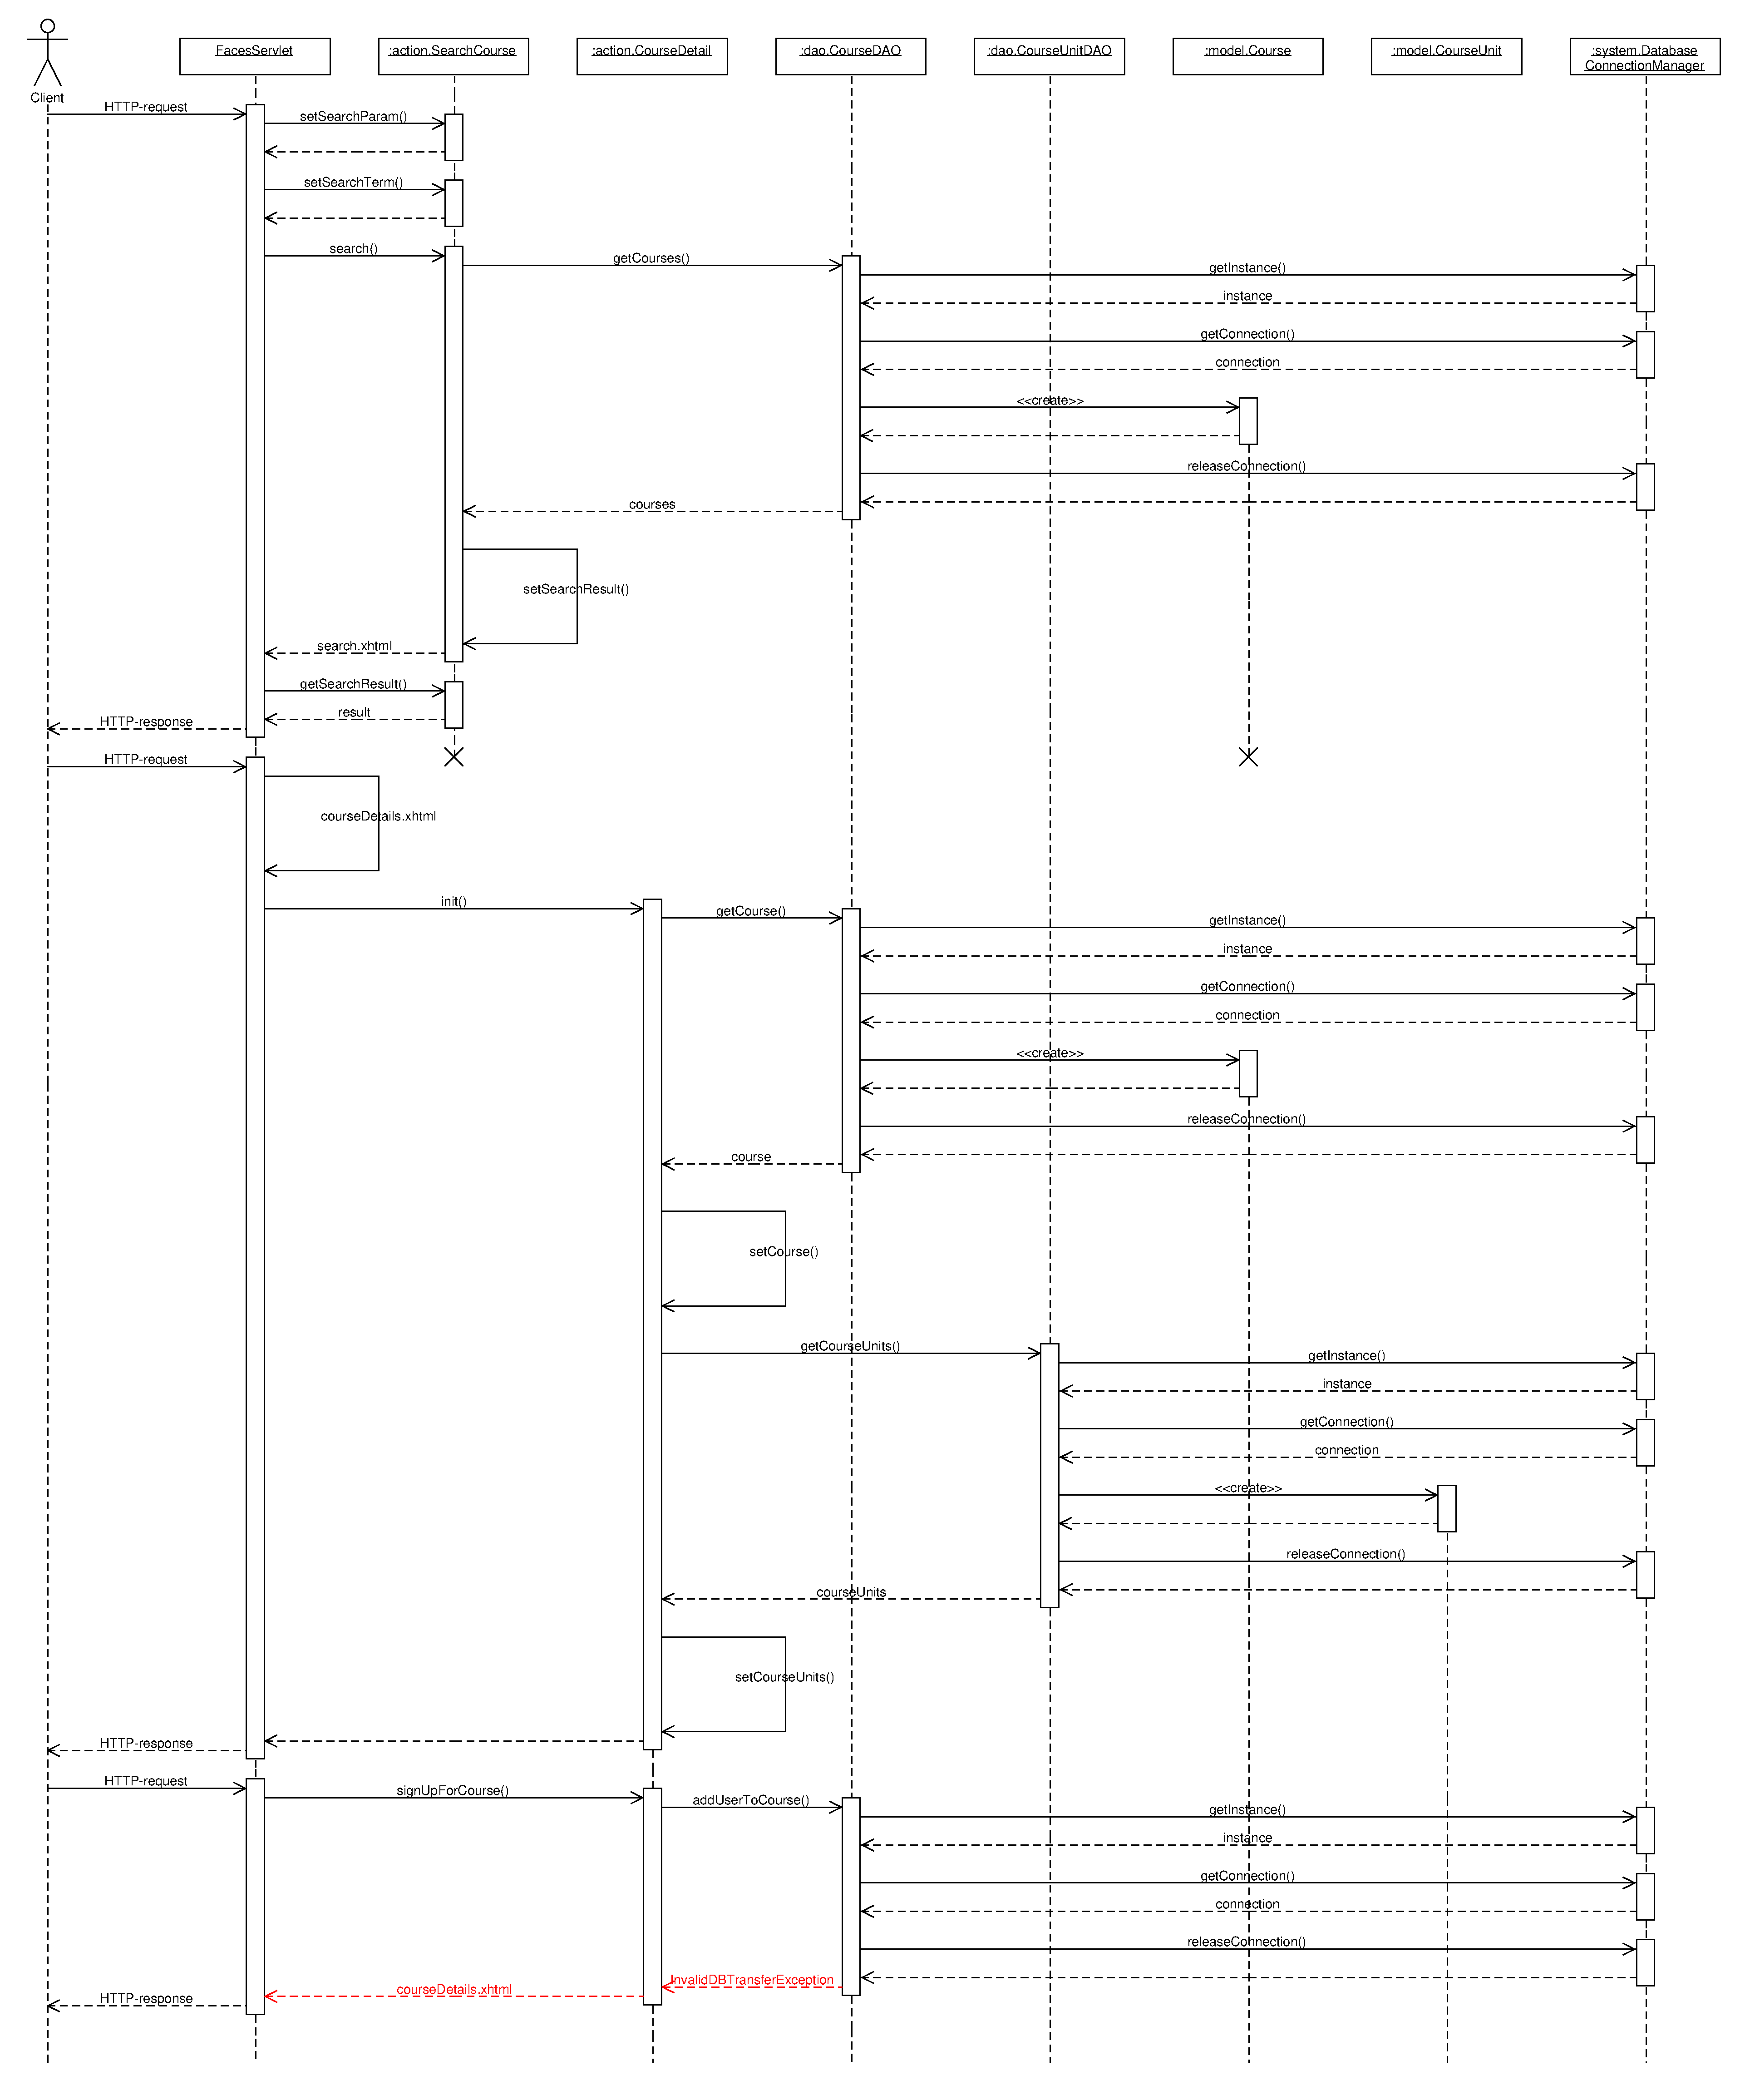
\includegraphics[scale=0.26]{./Grafiken/Sequenzdiagramm-Kursanmeldung.pdf}

\section{Konto aufladen}

\begin{tiny}
MB
\end{tiny}

Der eingeloggte Nutzer befindet sich auf der Seite \glqq buyCredits.xhtml\grqq{} zur Kontoaufladung. Dort werden alle relevanten Daten bezüglich der Kreditkarte angegeben, sowie der aufzuladene Betrag (siehe Kapitel 4.2.2 \glqq buyCredits.xhtml\grqq{}). Nach erfolgreicher Aufladung wird eine Bestätigung angezeigt.

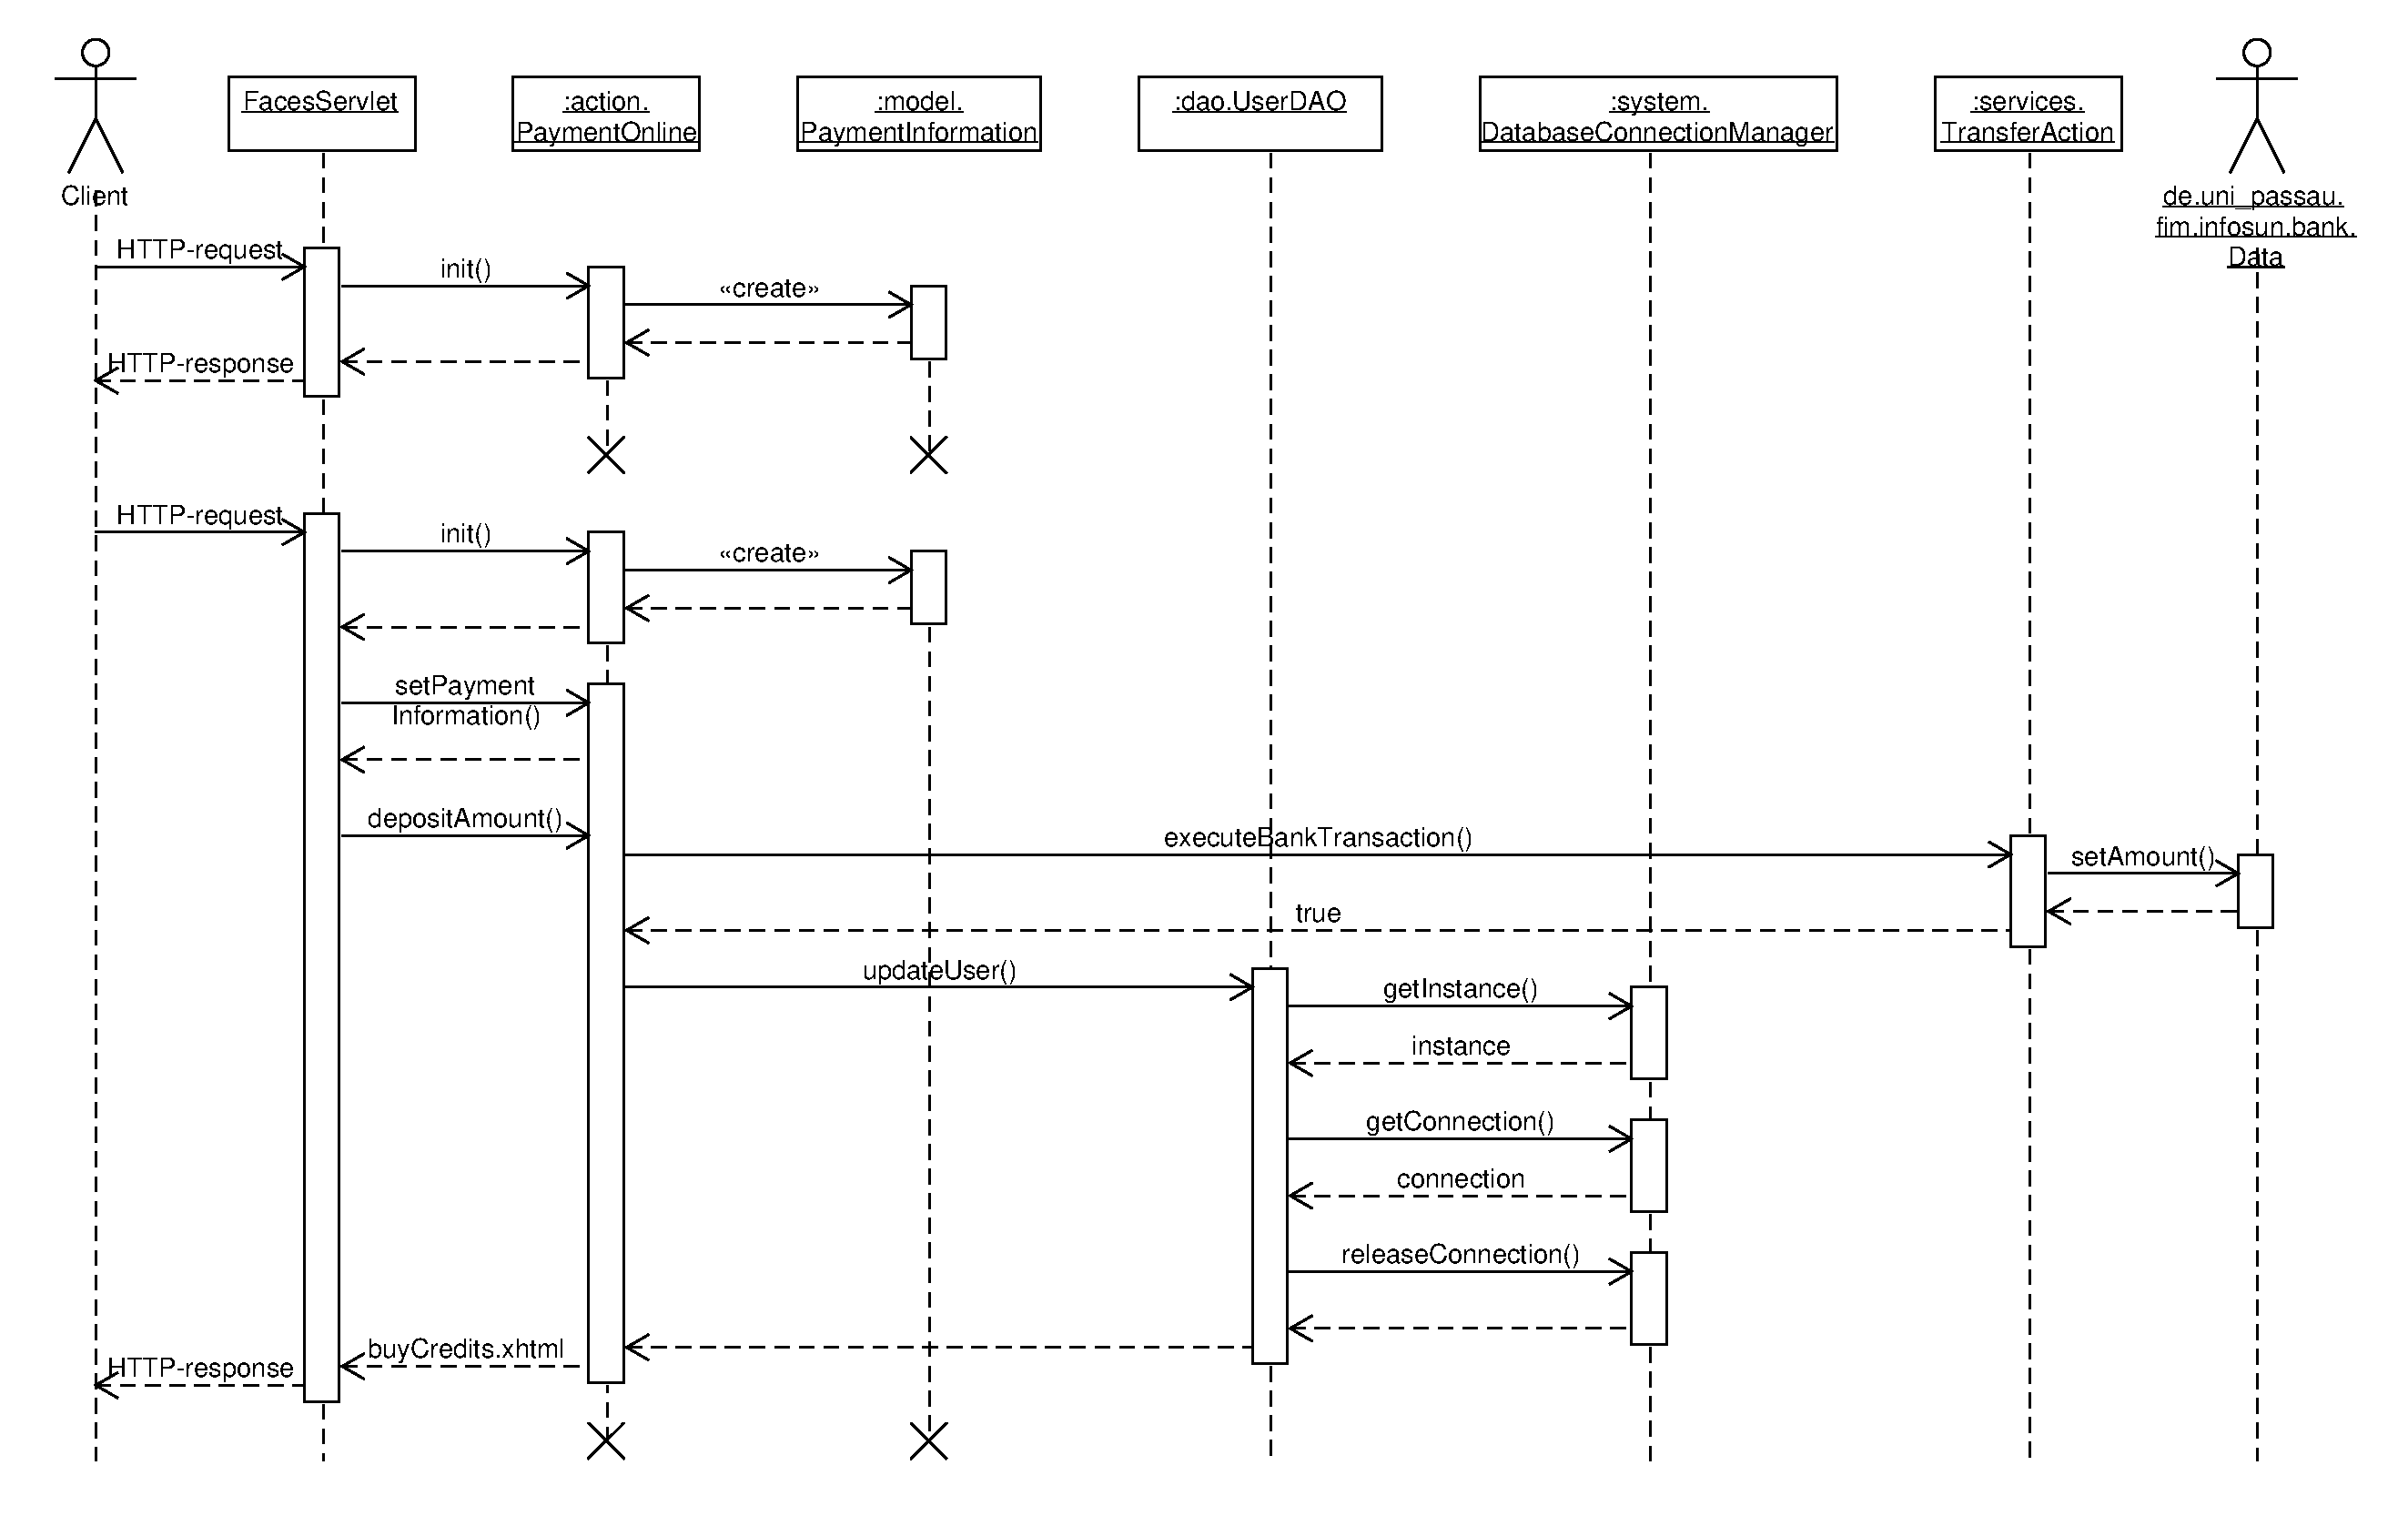
\includegraphics[scale=0.45]{./Grafiken/Sequenzdiagramm-KontoAufladung.pdf}
\chapter{ER-Modell}

\begin{tiny}
PC
\end{tiny}

\section{Diagramm}

In diesem Kapitel werden die systeminternen Entitäten und deren Relationen zueinander sowie alle dazugehörigen Attribute im nachfolgenden ER-Diagramm dargestellt und kurz beschrieben.

\includegraphics[scale=0.085]{./Grafiken/ER-Diagramm.pdf}

\section{Beschreibung}
\subsection{User}
Ein im System registrierter Nutzer, welcher entweder als einfacher registrierter Nutzer, oder zusätzlich als Kursleiter, Administrator, oder auch beides gespeichert wird und anhand der 'ID' eindeutig identifizierbar ist. Ein User kann eine Adresse angeben (vgl. 'Address'). Zusätzlich werden die gezahlten Beiträge des Nutzers zusammen mit dem Buchungsdatum in der systeminternen Geldstatistik gespeichert, sofern sich dieser zu zahlungspflichtigen Kurseinheiten (vgl. 'Course unit') angemeldet hat. Ein User kann an beliebig vielen Kursen (vgl. 'Course') und Kurseinheiten teilnehmen. Die Attribute 'E-mail verification' bzw. 'Admin verification' prüfen, ob der Nutzer über seinen persönlichen E-mail Account bzw. durch einen Administrator verifiziert wurde.

\subsection{Course Instructor}
Ein registrierter Nutzer, welcher im System als Kursleiter gespeichert und anhand seiner 'ID' eindeutig identifizierbar ist. Ein 'Course instructor' kann beliebig viele Kurse leiten (vgl. 'Course').

\subsection{System admin}
Ein registrierter Nutzer, welcher im System als Systemadministrator gespeichert ist und anhand seiner 'ID' eindeutig identifizierbar ist. Ein 'System admin' kann sowohl beliebig viele Systemattribute (vgl. 'System attributes') editieren als auch beliebig die Gestaltung der Webanwendung anpassen (vgl. 'Customization data').

\subsection{Address}
Die Anschrift eines registrierten Nutzers bzw. einer Kurseinheit (vgl. 'Course unit'). Diese ist durch ihre 'ID' eindeutig identifizierbar und kann entweder genau einem 'User' oder genau einer 'Course unit' zugeordnet werden.

\subsection{System attributes}
Enthält vom Systemadministrator festgelegte Attribute, welche der Funktionalität der Webanwendung dienen. Diese können bei Bedarf von allen im System gespeicherten Administratoren editiert werden.

\subsection{Customization data}
Enthält den Titel der Webanwendung ('System title'), den Titel der CSS-Datei ('CSS') und kann bei Bedarf von allen im System gespeicherten Administratoren editiert werden.

\subsection{Course}
Ein angebotener Kurs zudem sich beliebig viele Nutzer anmelden können und von mindestens einem 'Course instructor' geleitet wird. Ein 'Course' kann beliebig viele Kurseinheiten (vgl. 'Course units') anbieten und ist anhand der 'ID' eindeutig identifizierbar. Zusätzlich werden die gezahlten Beiträge innerhalb eines Kurses in der systeminternen Geldstatistik (vgl. 'Statistics') gespeichert. Das Attribut 'User To Be Informed' beschreibt, ob ein Nutzer Nachrichten zu einem Kurs abonniert hat zu dem er angemeldet ist.

\subsection{Course unit}
Eine Kurseinheit, welche innerhalb genau eines Kurses (vgl. 'Course') angeboten wird und anhand seiner 'ID' eindeutig identifizierbar ist. Sie hat genau eine Anschrift (vgl. 'Address'). An einer Kurseinheit können beliebig viele Nutzer teilnehmen, vorausgesetzt die maximale Teilnehmerzahl ('max. participants') ist noch nicht erreicht. 

\end{document}
